%%%%%Präambel%%%%%

\documentclass[12pt,a4paper]{article}%Schriftgröße, Papierformat einstellen
%\documentclass{scrbook}
\usepackage[top=30mm,bottom=30mm]{geometry}
\usepackage{lipsum}
\usepackage{csquotes}
%Pakete laden zur deutschen Rechtschreibung und für Umlaute
\usepackage[T1]{fontenc}
\usepackage[ngerman]{babel}
\usepackage[utf8]{inputenc} %für Windows, Linux
%\usepackage[applemac]{inputenc} %für Mac
%\usepackage{xcolor}
\usepackage{graphicx}
\usepackage{caption}
\usepackage[dvipsnames]{xcolor}
\usepackage{cancel}
\usepackage{titlesec}
\usepackage{cite}
\usepackage{filecontents}
\usepackage{tabularx}
\usepackage{harvard}
\usepackage{units}
\usepackage{longtable} 
\usepackage{multirow}
\usepackage{chngcntr}
\usepackage{stmaryrd}
\usepackage{array}
\usepackage{autobreak}
\usepackage{booktabs}
\usepackage{float}
\usepackage{wrapfig}
\usepackage{hhline}
\let\harvardleftorig\harvardleft
%\usepackage[round]{natbib}
%\usepackage{hyperref}
\usepackage[nottoc,numbib]{tocbibind}

%Pakete laden zu mathematischen Symbolen etc.
\usepackage{calc} 
\usepackage{amsmath,amssymb,amsthm,amsopn}
\usepackage{scrpage2}
\pagestyle{scrheadings}
\clearscrheadfoot
\automark[chapter]{section}
\ofoot{\pagemark}
\ifoot{}
\chead{\headmark}
\setfootsepline{1pt}
\setheadsepline{1pt}
%\setheadsepline[\textwidth+20pt]{0.5pt}

\DeclareMathOperator{\grad}{grad}
\DeclareMathOperator{\diverg}{div}
\DeclareMathOperator{\rot}{rot}
\DeclareMathOperator{\spur}{spur}
\DeclareMathOperator{\determ}{det}

%Inhaltsverzeichnis mit Links erstellen
\usepackage[colorlinks,
pdfpagelabels,
pdfstartview = FitH,
bookmarksopen = true,
bookmarksnumbered = true,
linkcolor = black,
plainpages = false,
hypertexnames = false,
citecolor = black] {hyperref}

% Umgebungen für Definitionen, Sätze, usw.
\newtheorem{satz}{Satz}[section]
\newtheorem{definition}[satz]{Definition}     
\newtheorem{lemma}[satz]{Lemma}	
\newtheorem{bem}{Bemerkung}[section]
% Es werden Sätze, Definitionen etc innerhalb einer Section mit
% 1.1, 1.2 etc durchnummeriert, ebenso die Gleichungen mit (1.1), (1.2) ..                  
\numberwithin{equation}{section}

\setcounter{secnumdepth}{4}
\setcounter{tocdepth}{4}

\titleformat{\paragraph}
{\normalfont\normalsize\bfseries}{\theparagraph}{1em}{}
\titlespacing*{\paragraph}
{0pt}{3.25ex plus 1ex minus .2ex}{1.5ex plus .2ex}

%neue Befehle definieren
\newcommand{\R}{\mathbb{R}} %zB \R als Abkürzung für das Symbol der reellen Zahlen
\newcommand{\N}{\mathbb{N}}
\newcommand{\Z}{\mathbb{Z}}
\newcommand{\Q}{\mathbb{Q}}
\newcommand{\C}{\mathbb{C}}
\newcommand{\diffp}{\partial}
\newcommand{\laplace}{\Delta}

\newcommand{\subsubsubsection}{\paragraph}
\newcommand\citevgl
{\def\harvardleft{(vgl.\ \global\let\harvardleft\harvardleftorig}%
 \cite
}
\newcommand\citeVgl
{\def\harvardleft{(Vgl.\ \global\let\harvardleft\harvardleftorig}%
 \cite
}

\newcommand{\tabitem}{~~\llap{\textbullet}~~}

\def\ccite#1#2{\glqq #1\grqq\cite{#2}}

\newcolumntype{L}[1]{>{\raggedleft\let\newline\\\arraybackslash\hspace{0pt}}m{#1}}
%Makros
%Makro Color
%#1 Text
\def\colBord#1{\begingroup\color{Fuchsia}{#1}\endgroup}
\def\colRed#1{\begingroup\color{Red}{#1}\endgroup}
\def\colGreen#1{\begingroup\color{LimeGreen}{#1}\endgroup}
\def\colBlue#1{\begingroup\color{NavyBlue}{#1}\endgroup}

\def\usGreen#1#2{\underset{\colGreen{#1}}{#2}}
\def\usBord#1#2{\underset{\colBord{#1}}{#2}}

\def\ubGreen#1#2{\underbrace{#2}_{\colGreen{#1}}}

\def\defF{\textbf{Def.: }}
\def\mDef#1{
\begin{definition}
  #1
\end{definition}}

\def\vecT#1{\left(\begin{array}{c} #1 \end{array}\right)}
\def\dddot{\cdot \\ \cdot \\ \cdot}
\def\vecD#1{\vecT{#1_1 \\ \dddot \\ #1_d}}
\def\vecDt#1#2{\vecT{#1 \\ \dddot \\ #2}}
\def\vecN{\mathcal{O}}
\def\vspan#1{span \lbrace #1 \rbrace}
\def\vdim#1{dim \lbrace #1 \rbrace}
\def\vker#1{ker \lbrace #1 \rbrace}
\def\vrang#1{Rang \lbrace #1 \rbrace}
\def\mzxz#1#2#3#4{\left(\begin{array}{c c} #1 & #2 \\ #3 & #4 \\ \end{array}\right)}
\def\mdxd#1#2#3{\left(\begin{array}{c c c} #1 \\ #2 \\ #3 \end{array}\right)}
\def\dfp#1#2{\frac{\partial #1}{\partial #2}}
\def\diff#1#2{\frac{\mathrm{d}#1}{\mathrm{d}#2}}

\def\epsF{\pmb{\varepsilon}}

\def\multiTwo#1#2{\multicolumn{2}{>{\hsize=\dimexpr2\hsize+2\tabcolsep+\arrayrulewidth\relax}#1}{#2}}
\def\multiThree#1#2{\multicolumn{3}{>{\hsize=\dimexpr3\hsize+4\tabcolsep+2\arrayrulewidth\relax}#1}{#2}}

\def\inR#1{\qquad ,\; #1 \in \R}
\def\inRs{\in \R}
\def\bracks#1{\left[ #1 \right]}
\def\abs#1{\left| #1 \right|}
\def\brac#1{\left( #1 \right)}

%laziness
\def\fermi{Fermi-Dirac-Verteilung}

\newcolumntype{L}[1]{>{\raggedleft\let\newline\\\arraybackslash\hspace{0pt}}m{#1}}
\newcolumntype{R}[1]{>{\raggedright\let\newline\\\arraybackslash\hspace{0pt}}m{#1}}



\def\formTab#1#2{
\begin{equation}
  \begin{tabularx}{12cm}{R{3cm} l l}
    #1 &: &$#2$
  \end{tabularx}
\end{equation}
}
\newcommand{\formTabL}[3]{
\begin{equation}
  \begin{tabularx}{12cm}{R{3cm} l l}
    #1 &: &$#2$ 
  \end{tabularx}
  \label{eq:#3}
\end{equation}}
\def\formTn{$ \\ $\;$ & $\;$ & $}
\def\formTnQ{$ \\ $\;$ & $\;$ & $\qquad}
\def\formTnQQ{$ \\ $\;$ & $\;$ & $\qquad \qquad}
\def\formTnQQQ{$ \\ $\;$ & $\;$ & $\qquad \qquad \qquad}

\renewcommand{\theequation}{\arabic{section}.\arabic{subsection}
.\arabic{equation}}
%Setzt den equation-Zaehler nach jeder Seite zurueck
\numberwithin{equation}{subsection}	


%\setlength\abovedisplayskip{0pt}

% Auf der Seite http://detexify.kirelabs.org/classify.html können Sie mathematische Symbole, Pfeile usw per Maus eingeben und bekommen den Latex-Befehl dafür angezeigt.
% detexify gibt es auch als App...

%jetzt beginnt das eigentliche Dokument
\begin{document}

\bibliographystyle{agsm}

\author{}
\title{\underline{HM1 Kurzzusammenfassung} \\ $\;$ \\ $\;$ \\ Florian Leuze}
\date{}

\maketitle % erzeugt den Kopf
\newpage

\tableofcontents

  \subsection*{Versionierung}
  \begin{tabular}{|p{2cm}|p{1cm}|p{1.5cm}|p{8.5cm}|}\hline
    Datum & Vers. & Kürzel & Änderung \\ \hline
    19.04.2018 & 0.1 & FL & Erzeugung Dokument; Erzeugung Inhaltsverzeichnis; Erzeugung Versionierung; Erzeugung 2.1 - 2.7.4 \\ \hline
    19.04.2018 & 0.2 & FL & Korrekturen 2.6.1 - 2.6.9 u. 2.7.1 - 2.7.2 Titel\\ \hline
    20.04.2018 & 0.2.1 & FL & Erzeugung 2.7.1.1 - 2.7.1.4; Korrektur Riemannsche Untersumme; Erzeugung Literaturverzeichnis \\ \hline
    01.05.2018 & 0.2.2 & FL & Neustrukturierung; Erzeugung Allgemeines; Erzeugung Zahlen \\ \hline
    01.08.2018 & 0.3.0 & FL & Überarbeitung Trigonometrie \\ \hline
    04.08.2018 & 0.3.1 & FL & Erzeugung lin. skal. Diffgleichungen, LGS \\ \hline
    05.08.2018 & 0.3.2 & FL & Erzeugung Analytische Geometrie; Erzeugung Logik und Beweise \\ \hline
    06.08.2018 & 0.3.3 & FL & Erzeugung Mengen, Relationen und Abbildungen, Erzeugung konvergente Folgen \\ \hline
    07.08.2018 & 0.3.4 & FL & Erzeugung el. realw. Funktionen, Ableitung; Fertigstellung konvergente Folgen \\ \hline
    08.08.2018 & 0.3.5 & FL & Erzeugung Ableitung, Taylorpolynome und Reihen. \\ \hline
    09.08.2018 & 0.4.0 & FL & Umordnung von Reihen, Stetigkeit, Extremalprobleme, Funktionenfolgen; Korrekturen am Layout \\ \hline
    09.08.2018 & 0.4.2 & FL & Korrekturen am Layout \\ \hline
    09.08.2018 & 0.4.3 & FL & Korrektur Def.7.8 \\ \hline
  \end{tabular}
\newpage
\listoffigures

\newpage

\section{Allgemeines}
	\subsection{Trigonometrie}
	  \subsubsection{Winkelfunktionen}
	  \begin{align}
	    sin(\alpha) = \frac{Gegenkathete}{Hypothenuse}\\
	    cos(\alpha) = \frac{Ankathete}{Hypothenuse}\\
	    tan(\alpha) = \frac{Gegenkathete}{Ankathete} \label{eq:trigo_Winkelf}
	  \end{align}
	  
	  \subsubsubsection{Wichtige Werte}
	  \renewcommand{\arraystretch}{1.5}
	  \begin{tabular}{|p{3.2cm}|p{1.8cm}|p{1.8cm}|p{1.8cm}|p{1.8cm}|p{1.8cm}|}\hline
		  $\alpha$ in Gradmaß & $0^{\circ}$ & $30^{\circ}$ & $45^{\circ}$ & $60^{\circ}$ & $90^{\circ}$ \\ \hline
		  $\alpha$ in Bogenmaß & $0$ & $\frac{\Pi}{6}$ & $\frac{\pi}{4}$ & $\frac{\pi}{3}$ & $\frac{\pi}{2}$ \\ \hline
		  $sin\alpha$ & $\frac{1}{2}\sqrt{0}$ & $\frac{1}{2}\sqrt{1}$ & $\frac{1}{2} \sqrt{2}$ & $\frac{1}{2}\sqrt{3}$ & $1$ \\ \hline
		  $cos\alpha$ & $1$ & $\frac{1}{2}\sqrt{3}$ & $\frac{1}{2}\sqrt{2}$ & $\frac{1}{2}\sqrt{1}$ & $\frac{1}{2}\sqrt{0}$ \\ \hline
		  $tan\alpha$ & $0$ & $\frac{1}{3}\sqrt{3}$ & $1$ & $\sqrt{3}$ & n.d. \\ \hline
	  \end{tabular}
	  \renewcommand{\arraystretch}{1}
	  
	  \subsubsection{Sinussatz}
	  \begin{equation}
	    \frac{a}{sin\alpha} = \frac{b}{sin\beta} = \frac{c}{sin\gamma} = 2r = \frac{abc}{2F} \label{eq:allg_sinussatz}  
	  \end{equation}
	  
	  \subsubsection{Cosinussatz}
	  \begin{align}   
	    a^2 = b^2 + c^2 - 2bc cos\alpha\\
	    b^2 = c^2 + a^2 - 2ca cos\beta\\
	    c^2 = a^2 + b^2 - 2ab cos\gamma \label{eq:trigo_cosinussatz}
	  \end{align}
	  
	  \subsubsection{Tangenssatz}
	  \begin{align}
	    \frac{b + c}{b - c} = \frac{tan\left(\frac{\beta + \gamma}{2}\right)}{tan\left(\frac{\beta - \gamma}{2}\right)} 
	    = \frac{cot\left(\frac{\alpha}{2} \right)}{tan\left(\frac{\beta - \gamma}{2}\right)}
	  \end{align}
	  Analog für $\frac{a + b}{a - b}$ und $\frac{a + c}{a - c}$.\label{eq:trigo_tangenssatz}
	  
	  \subsubsection{Umwandlung}
	  \begin{align}
	    tan\alpha = \frac{sin\alpha}{cos\alpha}\\
	    sin^2(\alpha) + cos^2(\alpha) = 1\\
	    1 + tan^2(\alpha) = \frac{1}{cos^2(\alpha)} = sec^2(\alpha)\\
	    1 + cot^2(\alpha) = \frac{1}{sin^2(\alpha)} = csc^2(\alpha)\label{eq:trigo_umwandlung}
	  \end{align}
	  
	  \subsubsection{Additionstheoreme}
	  \begin{align}
	    sin(x \pm y) &= sin(x) cos(y) \pm cos(x) sin(y)\\
	    cos(x \pm y) &= cos(x) cos(y) \mp sin(x) sin(y)\\\\
	    tan(x \pm y) &= \frac{tan(x) \pm tan(y)}{1 \mp tan(x) tan(y)} = \frac{sin(x \pm y)}{cos(x \pm y)}\\
	    cot(x \pm y) &= \frac{cot(x) cot(y) \mp 1}{cot(y) \pm cot(x)} = \frac{cos(x \pm y)}{sin(x \pm y)}\\\\
	    sin(x + y) \cdot sin(x - y) &= cos^2(y) - cos^2(x) = sin^2(x) - sin^2(y)\\
	    cos(x + y) \cdot cos(x - y) &= cos^2(y) - sin^2(x) = cos^2(x) - sin^2(y)\label{eq:trigo_addtheo}
	  \end{align}
	  
	  \subsubsection{Folgerungen aus den Additionstheoremen}
	  \begin{align}
	  cos^2(\frac{x}{2}) + sin^2(\frac{x}{2}) &\;\;= cos(\frac{x}{2}) cos(\frac{x}{2}) + sin(\frac{x}{2}) sin(\frac{x}{2})\\ 
	  &\overset{\eqref{eq:trigo_addtheo}}{=} cos(\frac{x}{2}-\frac{x}{2}) = cos(0) = 1\\
	  \\
	  2sin(\frac{x}{2})cos(\frac{x}{2}) &\;\;= sin(\frac{x}{2})cos(\frac{x}{2}) + sin(\frac{x}{2})cos(\frac{x}{2})\\
	  &\overset{\eqref{eq:trigo_addtheo}}{=} sin(\frac{x}{2}+ \frac{x}{2}) = sin(x)\\
	  \\
	  sin(2x) = sin(x+x) &\overset{\eqref{eq:trigo_addtheo}}{=} sin(x)cos(x) + sin(x)cos(x) \\
	  &\;\;=2sin(x)cos(x) \label{eq:trigo:addtheo_folg}
	  \end{align}
	  \newpage

\section{Zahlen}
  \subsection{Zahlbereiche}
    \subsubsection{Natürliche Zahlen}
    \begin{itemize}
      \item Direkt vom Zählen abgeleitet.
      \item $\N = \{1, 2, 3, 4, ...\}$
      \item Gleichungen wie $n+x = m$ i.A. in $\N$ nicht lösbar. 
    \end{itemize}

    \subsubsection{Ganze Zahlen}
    \begin{itemize}
      \item $\Z = \{..., -3, -2, -1, 0, 1, 2, 3, ...\}$
      \item Gleichungen wie $n \cdot x = m$ i.A. in $\Z$ nicht lösbar.
    \end{itemize}

    \subsubsection{Rationale Zahlen}
		\begin{itemize} 
			\item $\Q = \left\lbrace \frac{m}{n}: n\in \N, m \in \Z\text{, m, n teilerfremd} \right\rbrace$
			\item Gleichungen wie $x^2 = 2$ in $\Q$ nicht lösbar.
		\end{itemize}

		\subsubsection{Reelle Zahlen}
		\begin{itemize}
			\item $\R = \left\lbrace x = \sum_{j = - \infty}^n x_j 10^j : x_j \in \{0, 1, ..., 9\}\; \text{für ein n} \in \Z \right\rbrace $
			\item Gleichungen wie $x^2 = -1$ in $\R$ nicht lösbar.
		\end{itemize}

		\subsubsection{Komplexe Zahlen}
		\begin{itemize}
			\item $\C = \left\lbrace z = x + iy:\; x,\;y \in \R \right\rbrace$
			\ $i$ heißt imaginäre Einheit, es gilt $\R \subset \C$.
		\end{itemize}
	
	\subsection{Algebraische Strukturen}
		\subsubsection{Gruppe}
		\begin{definition} 
		  \glqq Eine Menge $M$ mit der Verknüpfung $+:M\times M \rightarrow M$, deren Elemente die Eigenschaften $(G1) - (G3)$ erfüllen, heißt Gruppe. Gilt zusätzlich $(G4)$, so heißt $(M,+)$ eine kommutative Gruppe.\grqq \cite{HM12}
		In der Literatur findet man als alternative Bezeichnung kommutativ auch abelsch. \citeVgl{LinAF}
		\end{definition}
		
			\subsubsubsection{Gruppenaxiome}
		  \begin{equation}
			  \begin{tabularx}{14.7cm}{l l l}
					(\textbf{G1}) & $x+(y+z) = (x+y)+z$ & \colBlue{(Assoziativgesetz)}\\
					(\textbf{G2}) & $x+0 = x = 0+x$ & \colBlue{(0 ist das neutrale Element)}\\
					(\textbf{G3}) & $x+(-x) = (-x)+x = 0$ & \colBlue{(-x ist das inverse Element zu x)}\\
					(\textbf{G4}) & $x+y = y+x$ & \colBlue{(Kommutativität also Vertauschbarkeit)}\\
			  \end{tabularx}
			  \label{ax:groupaxioms}
			\end{equation}
			
			\begin{definition} 
			  \glqq Sei eine Gruppe eine Verknüpfung mit $\cdot$ und $G' \subset G$ eine nichtleere Teilmenge. $G'$ heißt eine Untergruppe, wenn für $a,\;b \in G'$ auch $a\cdot b \in G'$ und $a^{-1} \in G'$. \cite{LinAF}
			  \newline
			  Im Bezug auf Gruppen und Ringe spielen die Begrifflichkeiten Isomorphismus und Homomorphismus eine Rolle. Beide Begriffe leiten sich von Morphismus (Struktur bzw. Form), Homo (gleich im Sinne von ähnlich) und Iso (gleich im Sinne von identisch) ab. 
		  \end{definition}
		  
			\begin{definition} 
			  \glqq Sind $G$ und $H$ Gruppen mit Verknüpfungen $\cdot$ und $\times$, so heißt eine Abbildung $\varphi : G \rightarrow H$ Homomorphismus (von Gruppen), wenn
			\end{definition}
			
			\begin{equation}
			  \varphi (a \cdot b) = \varphi (a) \times \varphi (b) \qquad  \forall a,\;b \in G\text{. \cite{LinAF}}
			\end{equation}
			\newline
			Ein Homomorphismus heißt Isomorphismus wenn er bijektiv ist. \cite{LinAF}
		
		  \subsubsection{Ring}
		  \begin{definition}
		    Erfüllt eine Menge die Eigenschaften einer Gruppe, hat jedoch zwei Verknüpfungen (z.B. $(+,-)$) spricht man von einem Ring.
		\end{definition}
		
		  \subsubsection{Körper}
		  \begin{definition}
		    Erfüllt eine Menge die Eigenschaften eines Ringes und ist zusätzlich kommutativ spricht man von einem Körper. Ein Beispiel für einen Körper ist die algebraische Struktur der rationalen und reellen Zahlen. 
		  \end{definition}
		
	    \subsubsubsection{Körperaxiome}
		  \begin{equation}
				\begin{tabularx}{14.7cm}{l l l}
					(\textbf{K1}) & $x\cdot(y\cdot z) = (x\cdot y)\cdot z$ & \colBlue{(Assoziativgesetz)}\\
					(\textbf{K2}) & $x\cdot 1 = 1 \cdot x = x$ & \colBlue{(1 ist das neutrale Element)}\\
					(\textbf{K3}) & $x\cdot(\frac{1}{x}) = (\frac{1}{x}) \cdot x = 1$ & \colBlue{($\frac{1}{x}$ ist das inverse Element zu x)}\\
					(\textbf{K4}) & $x\cdot y = y\cdot x$ & \colBlue{(Kommutativität also Vertauschbarkeit)} \\
					(\textbf{D}) & $x \cdot (y+z) = x \cdot y + x \cdot z$ & \colBlue{(Kommutativität also Vertauschbarkeit)}\\
				\end{tabularx}
		    \label{ax:körperaxiome}
		  \end{equation}
		  \newline
		
      \begin{definition} 
        \glqq Eine Menge $M$ mit den Verknüpfungen $+:M\times M  \rightarrow M$ und $\cdot: M\times M \rightarrow M$, deren Elemente die Gesetze $(G1) - (G4)$, $(M1) - M4)$ und $(D)$ erfüllt, heißt Körper.\grqq \cite{HM12}
      \end{definition}
		
	\subsection{Komplexe Zahlen}
	\begin{align}
		\C = \{ z &= x + iy:\; x,\;y \in \R \}\\
		i^2 &= 1
	\end{align}
	Den Realteil einer komplexen Zahl $z$ bezeichnet man i.A. mit $x$, den Imaginärteil mit $y$.
	\begin{equation}
	  Re\{z\} = x \qquad Im\{z\} = y
	\end{equation}
	
	\begin{definition} 
	  \glqq Zwei komplexe Zahlen sind gleich, wenn ihre Real- und Imaginärteile gleich sind. \grqq \cite{HM12}
	\end{definition}
	
		\subsubsection{Betrag der komplexen Zahl}
		Da sich komplexe Zahlen geometrisch im $\R^2$ interpretieren lassen, kann aus beiden Teilen ein Betragspfeil gebildet werden.
		\begin{equation}
		  |z| = \sqrt{x^2 + y^2}
		\end{equation}
		
		\subsubsubsection{Eigenschaften}
  	\begin{align}
		  |z| &= 0\\
			|z| = 0 &\Leftrightarrow z = 0\\
			|z_1 \cdot z_2| &= |z_1| |z_2|\\
			|z_1 + z_2| &\leq |z_1| + |z_2| \quad \text{\colBlue{(Dreiecksungleichung)}}
		\end{align}
		
		\subsubsection{Komplex konjugierte Zahl}
		\begin{definition} 
		  \glqq $\overline{z} = x -iy$ heißt die zu $z = x + iy$ konjugiert komplexe Zahl. \grqq \cite{HM12}
		\end{definition}
		
		\subsubsubsection{Eigenschaften}
		\begin{align}
			\overline{\overline{z}} &= z \\
			\overline{z_1 + z_2} = \overline{z_1} + \overline{z_2},&\qquad \overline{z_1 \cdot z_2} = \overline{z_1} \cdot \overline{z_2} \\
			Re\{z\} = \frac{1}{2} /z + \overline{z}), &\qquad Im\{z\} = \frac{1}{2i} /z - \overline{z})\\
			|z| = \sqrt{z \overline{z}}, &\qquad z\overline{z} = x^2 + y^2
		\end{align}
			
		\subsubsection{Polarkoordinatendarstellung}
		\begin{align}
			z = x + iy &= |z|(cos\varphi + isin\varphi)\\
			\Rightarrow x = |z| cos\varphi, &\qquad \rightarrow y = |z| sin\varphi) \nonumber\\
			\Rightarrow tan \varphi &= \frac{sin \varphi}{cos \varphi} = \frac{x}{y}
		\end{align}
		
		Achtung. Die Umkehrfunktion von Tanges ist nicht eindeutig. Es gilt:
		
		\begin{align}
		\varphi = 
		\begin{cases} 
		    arctan(\frac{x}{y}) \qquad &,\; x > 0,\; y\geq 0\\
		    \frac{\pi}{2}  &,\;x = 0,\; y > 0\\
		    \pi + arctan(\frac{y}{x}) &,\; x < 0\\
		    \frac{3\pi}{2} &,\; x=0,\;y< 0\\
		    2\pi + arctan(\frac{y}{x}) &,\; x> 0,\; y < 0
		\end{cases}
		\end{align}
	
	  \subsubsection{Multiplikation}
	  \begin{align}
	  z_1 \cdot z_2 &\;\; = |z_1|(cos\varphi_1 + isin\varphi_1) \cdot |z_2| (cos\varphi_2 + isin\varphi_2)\\
	  &\overset{\eqref{eq:trigo_addtheo}}{=} |z_1| |z_2| (cos(\varphi_1 + \varphi_2) + isin(\varphi_1 + \varphi_2))\\
	  &\;\; \Rightarrow |z_1 \cdot z_2| = |z_1| |z_2| \qquad ,\; Winkel = \varphi_1 + \varphi_2 \label{eq:zahl_kompl_mult}
	  \end{align}
	  
	  \subsubsection{Formel von de Moivre}
	  Setzt man in \eqref{eq:zahl_kompl_mult} $z_1 = z_2 = z$ ein erhält man die Formel von de Moivre.
	  \begin{align}
	    z \cdot z &= z^2 = |z|^2 (cos(2\varphi) + isin(2\varphi)) &,\; bzw.&&\nonumber\\
	    z^n &= |z|^n(cos(n\varphi)  + isin(n \varphi)) &,\; bzw.&&\nonumber\\
	    z^n& = |z|^n(cos\varphi + isin\varphi)^n\nonumber\\
	    &\Rightarrow (cos\varphi + isin\varphi)^n = cos(n\varphi) + isin(n\varphi)
	  \end{align}
	
	  Mit der Eulerschen Formel erhält man $e^{i\varphi} := cos\varphi + isin\varphi$. Daraus folgt:
	  \begin{align}
	  (e^{i\varphi})^n &= e^{in\varphi} \\
	  e^{i(\varphi_1 + \varphi_2} &= e^{i\varphi_1} e^{i\varphi_2}\\
	  e^{-i\varphi} &= \frac{1}{e^{i\varphi}}\\
	  z_x = |z_x|e^{i\varphi_x} &\Rightarrow z_1 z_2 = |z_1| |z_2| e^{i(\varphi_1 + \varphi_2)}
	  \end{align}

  \subsection{Polynome}
  Ein komplexes Polynom hat die Form
  \begin{align}
    p(z) = \sum_{k=0}^n a_k z^k = a_n z^n + a_{n-1} z^{n-1} + ... + a_0 \\
    a_k \in \C \nonumber
  \end{align}
  Falls $a_n \neq 0$ gibt $n$ den Grad des Polynoms an.
  \newline
  \begin{definition} 
    \glqq Ist $p(z)$ ein reelles Polynom, d.h. $a_k \in \R$, dann ist mit $z\in \C$ auch 
  $\overline{z} \in \C$ eine Nullstelle, d.h. aus $p(z) = 0$ folgt $p(\overline{z}) = 0$, d.h. die
  Nullstellen sind konjugiert komplex zueinander. \grqq \cite{HM12}
  \end{definition}

	\subsubsection{Fundamentalsatz der Algebra}
	\begin{satz}
	  Jedes Polynom vom Grad $\geq$ 1 besitzt in $\C$ mindestens eine Nullstelle.     
	  \label{satz:fund_alg}
	\end{satz}
	  
  \subsubsection{Polynomdivision}
    Über Polynomdivision lassen sich Polynome in Linearfaktoren zerlege. 
    \begin{align}
      Bsp.:  \nonumber\\
      (2z^3 - 3z^2 -6z +6) : (z-2) = (2z^2 +z -4)\quad ,\text{ Rest: } -2 \nonumber\\
      \underset{\text{\rule{3cm}{0.4pt}}}{-(2z^3 - 4z^2)} \nonumber \\
      0 + z^2 - 6z + 6 \nonumber \\
      \qquad \underset{\text{\rule[5mm]{3cm}{0.4pt}}}{z^2-2z} \nonumber \\
    \end{align}
    
    Aus \ref{satz:fund_alg} folgt:
    \begin{satz}
      Jedes Polynom p vom Grad $n\geq 1$ lässt sich über $\C$ in Linearfaktoren zerlegen, d.h. es gibt Zahlen $z_K$, die Nullstellen von p sind, sodass
      \begin{align*}
        p(z) = a_n(z-z_1)(z-z_2).../z-z_n)
      \end{align*}
    \end{satz}
    
    \begin{satz} $\;$
      \begin{itemize}
        \item[a)]
          Besitzt ein Polynom p vom n-ten Grad n+1 Nullstellen, so ist p = 0
        \item[b)]
          Stimmen zwei Polynome p und q jeweils vom Grad n an n+1 Stellen überein, so ist p = q.
      \end{itemize}
    \end{satz}
    
  \subsection{Einheitswurzeln}
  Wurzeln der Form $z^n = 1$ können allgemein einfach bestimmt werden. Mit $|z^n| = |z|^n = 1$ folgt $|z| = 1$. Mit der eulerschen Identität folgt aus
  \begin{align*}
    z &= e^{i\varphi} = cos \varphi + i \; sin\varphi = 1 = 1 + 0 \cdot i\\
    &\Rightarrow n\varphi = 2 \pi k \quad ,k \in \Z\\
    &\Rightarrow \varphi = \frac{2\pi k}{n}\\
    &\Rightarrow z_0 = 1 e^{i\cdot 0},\quad z_1 = e^{i\frac{2\pi}{n}}, \quad ... z_n = e^{i\frac{k\pi}{n}}
  \end{align*}    
  Allgemein gilt mit $z^n = a$ und $\varphi = arccos\left(\frac{|z|}{Re\{z\}}\right)$:
  \begin{align}
    z_k = a^{\frac{1}{n}} \cdot \left(cos\left(\frac{\varphi + 2k\pi}{n}\right) + i\cdot sin\left(\frac{\varphi + 2k\pi}{n}\right)\right)
  \end{align}
  Bei reellen Polynomen sind dabei die Nullstellen komplex konjugiert zueinander.
  \newpage
  
\section{Lineare skalare Differentialgleichungen mit konstanten Koeffizienzen}
  \begin{definition}
    Lineare skalare Diff.gleichungen mit konst. Koeffizienten sind Gleichungen der bauart:
    \begin{align*}
      Ly(x) = a_n y^{(n)}(x)+a_{n-1}y^{(n-1)}(x)+...+a_1y'(x) + a_o y(x) = f(x)
    \end{align*}
  \end{definition}
  \subsection{Ansätze}
  \begin{itemize}
    \item[a)] Homogene Diff.gleichung:
    Mit $\lambda$ als einfache NST:
    \begin{equation}
      y(x) = e^{\displaystyle\lambda x} \label{eq:dgl_Ansatz_a}
    \end{equation}
    Mit $\lambda$ als $n$-fache NST:
    \begin{equation}
      f(x) = e^{\displaystyle\lambda x}, xe^{\displaystyle\lambda x}, ..., x^{n-1}e^{\displaystyle\lambda x} 
    \end{equation}
    Mit $\lambda = \alpha + \beta i$ (komplexe Nullstellen):
    \begin{equation}
      e^{\alpha x}cos(\beta x),\quad e^{\alpha x} sin(\beta x)
    \end{equation}
    \item[b)] Inhomogenität der Form $f(x) = p_k(x) e^{sx}$ mit $p_k(x)$ als ein Polynom $k$-ten Grades.
    \begin{equation}
      y_p(x) = R_k(x)e^{sx}x^q
    \end{equation}
    Mit $R_k(x) = a_kx^k+...+a_0$ und $q$ als Vielfachheit der Nullstelle $s$ (ist $s$ keine Nullstelle so ist $q = 0$ und damit $x^q = 1$).
    \item[c)] Inhomogenität der Form $cos(kx)$ oder $sin(kx)$.
    \begin{equation}
      yp(x) = (a cos(kx) + b sin(kx)) x^q
    \end{equation}
    Beispiel Umformung:
    \begin{align}
      f(x) &= sin(4x)\nonumber\\
      Mit \quad
      (1)\;\;\; e^{i\varphi} &= cos \varphi + i sin\varphi\nonumber \\
      und \quad
      (2)\; e^{-i\varphi} &= cos \varphi - i sin \varphi\nonumber\\
      folgt \;mit \;(1) + (2) \;&bzw.\; (1)-(2)\nonumber\\
      e^{i\varphi} + e^{-i\varphi} = 2\;cos\varphi \quad &bzw. \quad e^{i\varphi}-e^{-i\varphi} = 2 \; sin\varphi\nonumber\\
      \Rightarrow cos \varphi = \frac{1}{2} (e^{i\varphi}+e^{-i\varphi}) &\quad \Rightarrow sin \varphi = \frac{1}{2i} (e^{i\varphi}-e^{-i\varphi}),\quad \forall \varphi \in \R
    \end{align}
    $q$ im Ansatz gibt die Vielfachheit der NST $i \varphi$ im charackteristischen Polynom des homogenen Teils der Gleichung an.
    \item[d)] Inhomogenität der Form $q_k(x)e^{\alpha x} cos(\beta x)$ oder $q_k(x)e^{\alpha x} sin(\beta x)$
    \begin{equation}
      yp(x) = R_k(x)x^qe^{\alpha x}cos(\beta x) + \tilde{R}_k(x) x^qe^{\alpha x}cos{\beta x}
    \end{equation}
  \end{itemize}
  \subsection{Vorgehensweise}
    \begin{flalign*}
      &\textbf{Schritt 1: } \text{Ansatz wählen}&
    \end{flalign*}
    \begin{flalign*}
      &\textbf{Schritt 2: } \text{Ansatz einsetzen und charackteristisches Polynom bilden}& \\
      &\text{Beispiel:}&
    \end{flalign*}
    \begin{align*}
      &y'' + 3y'+2y = 0 \\
      &\overset{\eqref{eq:dgl_Ansatz_a}}{\Rightarrow} \left(e^{\lambda x}\right)'' + 3\left(e^{\lambda x}\right)' + 2e^{\lambda x} = 0 \\
      \left(e^{\lambda x}\right)' &\;\;= \lambda e^{\lambda x} \Rightarrow \left(e^{\lambda x}\right)'' = \lambda^2 e^{\lambda x} \\
      &\;\;\Rightarrow \lambda^2 + 3 \lambda + 2 = 0
    \end{align*}
    \begin{flalign*}
      &\textbf{Schritt 3.1: } \text{Nullstellen des char. Polynoms suchen und in Ansatz einsetzen}&\\
      &Beispiel:&
    \end{flalign*}
    \begin{align*}
      \lambda^2 + 3 \lambda + 2 = 0 \Rightarrow \lambda_1 = -2,\quad \lambda_2 = -1
    \end{align*}
    \begin{flalign*}
      &\textbf{Schritt 3.2: } \text{Gegebenenfalls komplexe NST in reale umwandeln}&\\
      &Beispiel:&
    \end{flalign*}
    \begin{align*}
      y(x) &= C_1 e^{-x+ix} + C_2 e^{-x-ix} \\
      \Rightarrow y(x) &= \tilde{C}_1e^{-x}cosx + \tilde{C}_2 e^{-x}sinx \qquad, \tilde{C}_1, \tilde{C}_2 \in \R
    \end{align*}
    \begin{flalign*}
      &\textbf{Schritt 4: } \text{Allgemeine Lösung aufstellen}&
    \end{flalign*}
    \begin{align*}
      \Rightarrow y(x) = C_1 e^{-2x} + C_2 e^{-x}\quad, C_1,C_2\in \R
    \end{align*}
    
    \newpage
    \subsubsection{Anfangswertproblem}
    Falls Anfangswerte vorhanden sind können an dieser Stelle die Konstanten Koeffizienten explizit bestimmt werden. \newline
    \begin{flalign*}
    &Beispiel:&
    \end{flalign*}
    \begin{align*}
	    y(0) &= 1,\;y'(0) = 0\\
	    y(t) &= C_1 e^{5t} + C_2 e^{-2t}\\
	    &\Rightarrow y(0) = C_1 e^{5\cdot 0} + C_2 e^{-2\cdot 0} = 1\\ 
      &\Rightarrow C_1 = 1-C_2\\
      y'(t)& = 5 C_1 e^{5t} -2 C_2 e^{-2t} \Rightarrow y'(0) = 5C_1 - 2C_2 = 0\\
      &\Rightarrow y'(0) = 0 = 5(1-C_2)-2C_2 \Rightarrow C_2 = \frac{5}{7}\\
      &\Rightarrow C_1 = 1-C_2 = 1- \frac{5}{7} = \frac{2}{7}\\
      \; \\
      &\Rightarrow y(t) = \frac{2}{7} e^{5t}+\frac{5}{7}e^{-2t}
    \end{align*}
    
    \subsubsection{Inhomogenität}
      \begin{flalign*}
        &\textbf{Schritt 1: } \text{Ansatz wählen}&
      \end{flalign*}
      \begin{flalign*}
        &\textbf{Schritt 2: } \text{Ansatz gegebenenfalls ableiten und in homogenen Teil einsetzen}&
      \end{flalign*}    
      \begin{flalign*}
        &\textbf{Schritt 3: } \text{Über Koeffizientenvergleich Vorfaktoren bestimmen}&
      \end{flalign*}    
      \begin{flalign*}
        &\textbf{Schritt 4: } \text{Allgemeine Lösung bilden}&
      \end{flalign*}    
      \begin{equation}
        y(x) = y_{hom}(x) + y_p(x)
      \end{equation}
      \begin{flalign*}
        &\textbf{Schritt 5: } \text{Gegebenenfalls Anfangswertproblem lösen}&
      \end{flalign*}    
      \newpage
    
\section{Lineare Gleichungssysteme}
  \subsection{Gauss Algorithmus}
  Siehe Kurzzusammenfassung HM2
  \begin{align}
	     \begin{array}{c c c c c c c c l}
	       \tilde{a}_{11} x_1 & + & \tilde{a}_{12} x_2 & + & \dots & + & \tilde{a}_{1n} x_n & = &  \tilde{b}_1 \\
	       \ddots &\;& \ddots &\;&\;&\;&\;&\;&\vdots\\
	       \; & \; & a^{(r)}_{rr}x_r &+& \dots &+& a^{(r)}_{rn}x_n &=& b_r\\
	       &\;&\;&\;&\;&\;& 0 & = & b^{(r)}_{r+1}\\
	       &\;&\;&\;&\;&\;& \; & \vdots & \;\\
	       &\;&\;&\;&\;&\;& 0 & = & b^{(r)}_{m}
	     \end{array}
	\end{align}
	\begin{definition}
	  Die Zahl $r$ heißt der Rang der Matrix A. Die Zahl $a_{11}$ heißt Pivotelement (Tendenziell eher die Zahlen $a_{11}$ bis $a_{rr}$ heißen Pivotelemente, aber so wie oben stehts im Script). 
	\end{definition}
	
	\subsubsection{Lößbarkeit}
	\begin{itemize}
	  \item[1. Fall: ]
	  Damit Lösungen existieren können, muss $b^{(r)}_{r+1} = ... = b^{(r)}_{m} = 0$ gelten, sonst existieren keine Lösungen. Das heißt es darf keine Zeile allgemein der Form $a = 0$ mit $-\infty < a < 0 \lor 0 < a < \infty$ existieren.
	  \item[2. Fall: ]
	    Ist $b^{(r)}_{r+1} = ... = b^{(r)}_{m} = 0$ und ist $r = n$, so existiert eine eindeutige Lösung. Das heißt es existieren gleich viele Unbekannte wie Zeilen und Fall 1 ist ausgeschlossen.
    \item[3. Fall: ]
    Ist $b^{(r)}_{r+1} = ... = b^{(r)}_{m} = 0$ und ist $r < n$, so existiert eine Schar von Lösungen. D.h. es kann eine Variable frei gewählt werden.
  \end{itemize}
	\newpage
	
\section{Analytische Geometrie}
  \subsection{Dreidimensionaler Raum}
  \begin{definition}
    Der dreidimensionale Raum ist durch $\R^3 = \R \times \R \times \R = \lbrace p_1, p_2, p_3: p_1, p_2, p_3 \in \R \rbrace$. Jeder Punkt $p\in \R^3$ ist eindeutig durch die Angabe seiner Koordinaten $p_1, p_2, p_3)$ bestimmt.
  \end{definition}
  \subsubsection{Abstand}
  \formTab{Euklidischer Abstand zweier Punkte}{d(P,Q)=\sqrt{(p_1-q_1)^2 + (p_2-q_2)^2 + (p_3 - q_3)^2}} 
  \subsubsection{Vektoren} 
  \formTab{Norm eines Vektors}{||x||_{\R^3} = \sqrt{x_1^2 + x_2^2 + x_3^2}}
  Vektoren können skalar multipliziert oder miteinander addiert werden:
  \begin{align}
    \lambda \vecT{x_1 \\ x_2 \\ x_3} &= \vecT{\lambda x_1 \\ \lambda x_2 \\ \lambda x_3}\\
    \vecT{x_1 \\ x_2 \\ x_3} + \vecT{y_1 \\ y_2 \\ y_3} &= \vecT{x_1 + y_1 \\ x_2 + y_2 \\ x_3 + y_3}
  \end{align}   
  \begin{definition}
    Die Koordinaten $P = (p_1, p_2, p_3)$ eines Punktes $p$ definieren den Ortsvektor $p$. Sind zwei Punkte $P,Q$ mit Ortsvektoren $p,q$ gegeben, so gilt 
    \begin{equation}
      d(P,Q) = ||p-q||
    \end{equation}   
  \end{definition}  
    
  \subsubsection{Skalarprodukt}
  Das Skalarprodukt projeziert einen Vektor $b$ auf einen Vektor $a$. Es ist im $\R^3$ definiert als:
  \begin{align}
    (a,b) = <a,b> &= a_1 b_1 + a_2 b_2 + a_3 b_3 \\
    &bzw. \nonumber \\
    (a,b) &= ||a|| \; ||b|| cos \phi
  \end{align}
  Weiterhin gilt:
  \begin{equation}
  ||x|| = \sqrt{x_1^2 + x_2^2 + x_3^2} = \left(\left<\vecT{x_1 \\ x_2 \\ x_3},\vecT{x_1 \\ x_2 \\ x_3}\right>\right)^{\frac{1}{2}} = (x,x)^{\frac{1}{2}}
  \end{equation}
  \begin{definition}
	  $a$ und $b$ heißen orthogonal, falls 
	  \begin{equation*}
	    (a,b) = 0 
	  \end{equation*}
  \end{definition}
  
  \subsubsection{Vektor- bzw. Kreuzprodukt}
  \begin{definition}
    Der Betrag des Vektorproduktes $a\times b$ ist gleich dem Flächeninhalt des von $a$ und $b$ aufgespannten Parallelogramms. Dies folgt direkt aus der Trigonometrie des Dreiecks.
    \begin{equation}
      A = ||a \times b||
    \end{equation}
    Es gilt:
    \begin{equation}
      ||a \times b|| = ||a|| \; ||b|| sin\phi
    \end{equation}    
    Das Vektorprodukt $a \times b$ steht senkrecht auf $a$ und $b$. Die Vektoren $a,b,a \times b$ bilden ein Rechtssystem. $a$: Daumen, $b$: Zeigefinger, $a \times b$: Mittelfinger der rechten Hand.
  Es gelten folgende Eigenschaften:
  \begin{itemize}
    \item[i)   ] $a \times a = 0$
    \item[ii)  ] $a \times b = -b \times a$
    \item[iii) ] $(\lambda a) \times b = \lambda (a \times b)$
    \item[iv)  ] $a \times (b+c) = a \times b + a \times c$
    \item[v)   ]
    \begin{align*}
      \text{Seien }e_1, e_2, e_3\text{ die Einheitsvektoren (siehe HM2) dann gilt:}\\
      e_1 \times e_2 = e_3, \quad e_2 \times e_3 = e_1, \quad e_3 \times e_1 = e_2
    \end{align*}
    \item[vi)   ]
    \begin{equation}
      a := \vecT{a_1 \\ a_2 \\ a_3},\; b := \vecT{b_1 \\ b_2 \\ b_3} \Rightarrow a \times b =  \vecT{a_2 b_3 - a_3 b_2 \\ a_3 b_1 - a_1 b_3 \\ a_1 b_2 - a_2 b_1} 
    \end{equation}
  \end{itemize}
  \end{definition}
  Es gilt die Cauchy-Schwarzsche Ungleichung:
  \begin{align}
    x,y \in \R^n_{\backslash \lbrace 0 \rbrace} &\nonumber \\
    |x \cdot y| &\leq ||x|| \; ||y|| \nonumber \\
    |x \cdot y| &= ||x|| \; ||y|| \Leftrightarrow x = \lambda y \quad, \lambda \in \R
  \end{align}
  
  \subsubsection{Spatprodukt}
  \begin{definition}
    Drei Vektoren $a,b,c$ spannen ein Volumen auf.
    \begin{equation}
      [a,b,c] = (a \times b, c)
    \end{equation}
  \end{definition}
  
  \subsection{Geraden im $\R^2$}
	  \subsubsection{Parameterdarstellung}
	  Die Parameterdarstellung einer Gerade im $\R^2$ ist gegeben mit:
	  \begin{align}
	    x &= a + \lambda(b-a)\quad, \lambda \in \R \nonumber \\
	    &\Rightarrow x = a + \lambda u
	  \end{align}
	  Wobei $u$ die Richtung der Gerade angibt und Richtungsvektor heißt. $a$ heißt Stützvektor.
	  \begin{figure}[htbp] 
		  \centering
		  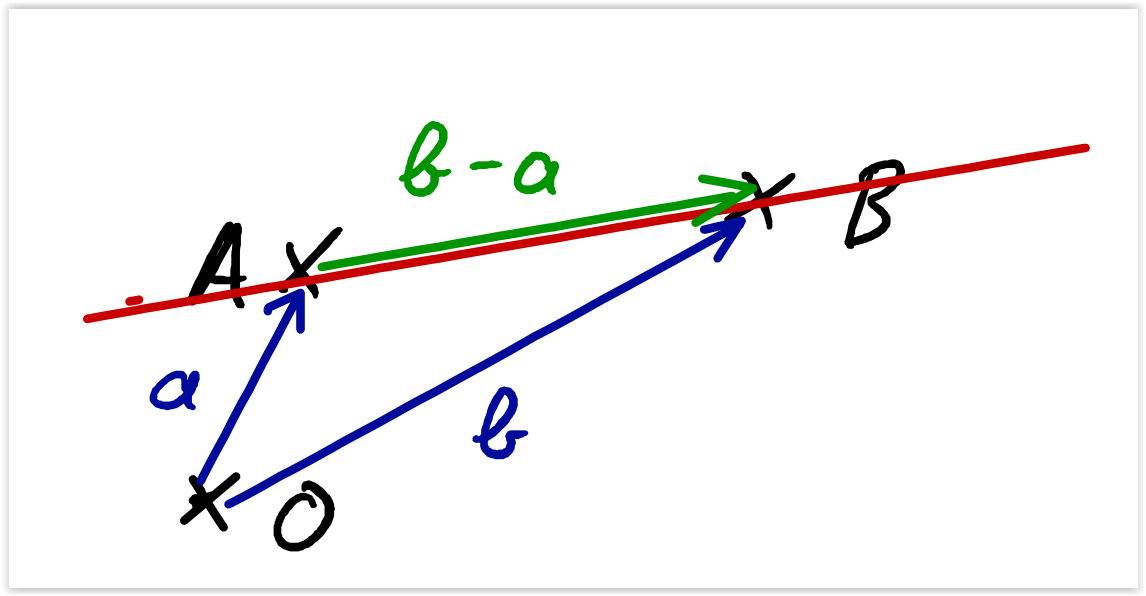
\includegraphics[width=0.7\textwidth]{Geraden.png}
		  \caption{Gerade im $\R^2$\protect\cite{HM12}}
		  \label{fig:gerade_R2}
	  \end{figure}

    \subsubsection{Darstellung in Gleichungs- bzw. Normalform}
    Zur Darstellung in der Normalform muss zunächst ein Normalenvektor $n$ der orthogonal auf $u$ steht gewählt werden, d.h. es muss gelten $(n,u) = 0$.
    \begin{align}
      (n,x) = (n,a + \lambda u) = (n,a) + \lambda \underbrace{(n,u)}_{=0} = (n,a) =: p
    \end{align}
    Die Gleichungsdarstellung ist dann:
    \begin{equation}
      (n,x)-p = 0 
    \end{equation}
    \subsubsection{Hessesche Normalform}
    Zur Bildung der Hesseschen Normalform wird der Normalevektor normiert und es muss $p \geq 0)$ gelten. 
    \begin{equation}
      \left(\frac{n}{||n||},x\right)-p = (n^*,x)-p = 0
    \end{equation}
    \subsubsection{Minimaler Abstand}
    Der Punkt mit minimalem Abstand zum Ursprung $x^*$ auf der Gerade ist der Punkt, an dem der Ortsvektor orthogonal auf der Gerade steht. Das einsetzen dieses Punktes in die Hessesche Normalform liefert also den Abstand zum Ursprung mit:
    \begin{equation}
    (n^*,x^*)=||x^*|| = p = Abstand
    \end{equation}
    \subsubsection{Abstand eines Punktes zur Gerade}
    $\tilde{x}$ sei ein beliebiger Punkt, dann ist
    \begin{equation}
      d = (n^*, \tilde{x})-p
    \end{equation}
    Der Abstand des Punktes zur Geraden.
  \subsection{Geraden und Ebenen im $\R^3$}
    \subsubsection{Parameterdarstellung einer Geraden im $\R^3$}
    \begin{align}
      &g: x = a + \lambda u \quad ,bzw. \nonumber \\
      &g: \vecT{x_1 \\ x_2 \\ x_3} = \vecT{a_1 \\ a_2 \\ a_3} + \lambda \vecT{u_1 \\ u_2 \\ u_3}
    \end{align}
    \subsubsection{Koordinatendarstellung einer Geraden im $\R^3$}
    Eine Gerade lässt sich im $\R^3$ auch als Schnittgerade zweier Ebenengleichungen ausdrücken. Ein Beispiel dazu:
    \begin{align*}
      g: &= \vecT{x_1 \\ x_2 \\ x_3} = \vecT{1 \\ 0 \\ 2} + \lambda \vecT{1\\2\\1} \\
      &\Rightarrow
      \begin{array}{l l l}
        x_1 = 1 + \lambda \\
        x_2 = 2\lambda \\
        x_3 = 2 + \lambda
      \end{array}
      \Rightarrow \lambda = \frac{x_2}{2}\\
      &\Rightarrow x_1 = 1 + \frac{x_2}{2},\quad x3 = 2 + \frac{x_2}{2}
    \end{align*}
    \subsubsection{Parameterdarstellung einer Ebene im $\R^3$}
    \begin{align}
      &E: x = a + \lambda u + \mu v \quad ,bzw. \nonumber \\
      &E: \vecT{x_1 \\ x_2 \\ x_3} = \vecT{a_1 \\ a_2 \\ a_3} + \lambda \vecT{u_1 \\ u_2 \\ u_3} + \mu \vecT{v_1 \\ v_2 \\ v_3}
    \end{align}        
    \subsubsection{Gleichungsdarstellung bzw. Hessesche Normalform einer Ebene im $\R^3$}
    \begin{align}
    &(n^*,x) = (n^*,a) + \lambda \underbrace{(n,u)}_{=0} + \mu \underbrace{(n,v)}_{=0} \nonumber \\
    &\Rightarrow (n^*,x) - (n^*,a) = 0 \quad mit \; (n,a) =: p \nonumber \\
    &\Rightarrow (n^*,x) - p = 0
    \end{align}
    $p$ gibt den Abstand der Gerade zum Ursprung an. $n$ muss auf beiden Richtungsvektoren  senkrecht stehen und lässt sich durch
    \begin{equation}
      n = \frac{u \times v}{|| u \times v||}
    \end{equation}
    bestimmen.
  
    \begin{figure}[htbp] 
		  \centering
		  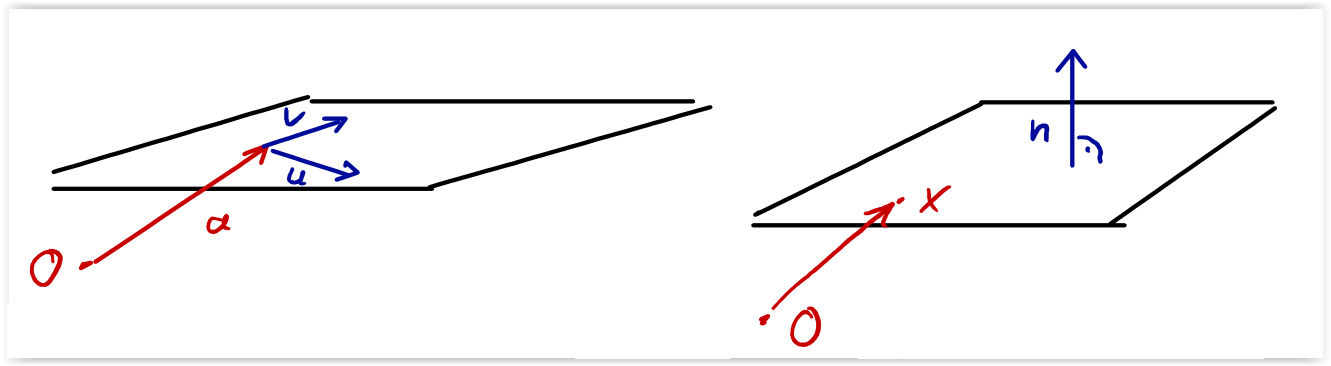
\includegraphics[width=0.7\textwidth]{Ebene_R3.png}
		  \caption{Ebenen im $\R^3$\protect\cite{HM12}}
		  \label{fig:ebene_R3}
	  \end{figure}
	  
	\subsection{Schnitte}
	  \subsubsection{Schnitt zweier Ebenen}
	  Sind die Normalenvektoren nicht parallel existiert eine Schnittgerade. Sie kann durch die entsprechenden Ebenengleichungen beschrieben werden.
	  \begin{align*}
	    E_1 &= \lbrace x\in \R^3:x_1 + 4x_2 = 2 \rbrace \\
	    E_2 &= \lbrace x \in \R^3: x_2 - x_3 = 1\rbrace \\
	    &\Rightarrow n_1 = \vecT{1\\4\\0},\quad n_2 = \vecT{0\\2\\-1} \\ 
	    &\Rightarrow n_1 \; und \; n_2 \;\text{nicht parallel} \Rightarrow \text{Schnittgerade ex.}\\
	    &\Rightarrow g=\lbrace x\in \R^3: x_1 + 4x_2 = 2, x_2 - x_3 = 1\rbrace
	  \end{align*}
	  Der Schnittwinkel zweier Ebenen kann über die jeweiligen Normalenvektoren bestimmt werden.
	  \begin{figure}[htbp] 
		  \centering
		  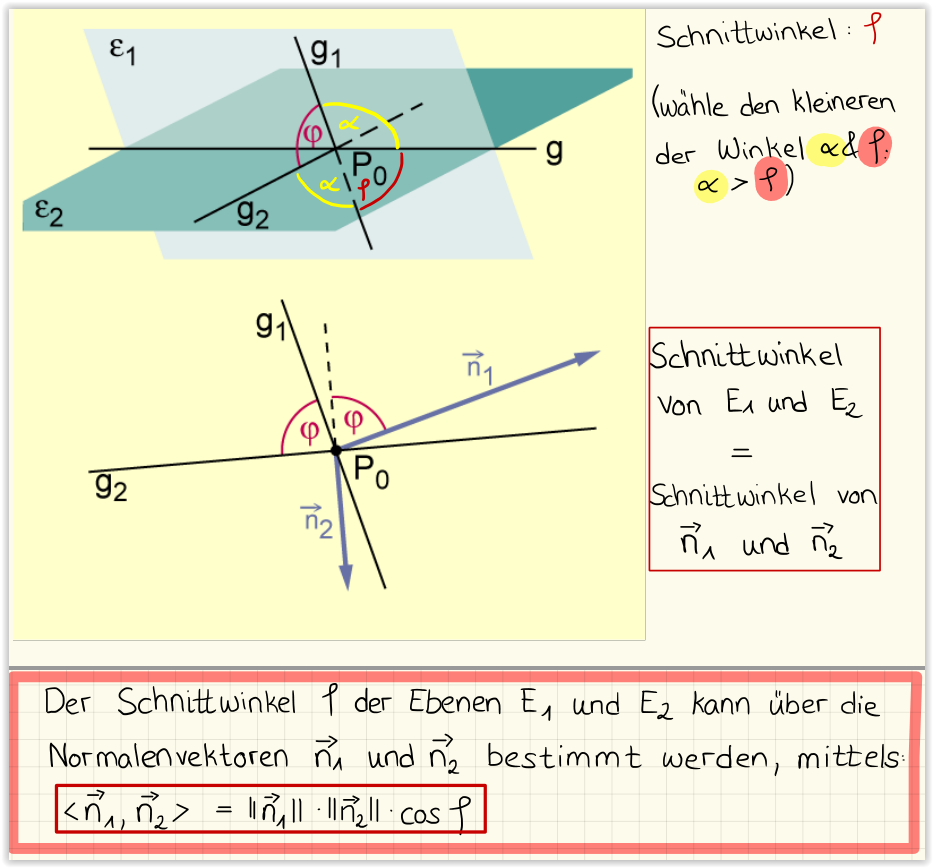
\includegraphics[width=0.67\textwidth]{schnitt_ebene.png}
		  \caption{Schnittwinkel zweier Ebenen\protect\cite{HM1Vortragsubung}}
		  \label{fig:ebene_schnittwinkel}
	  \end{figure} 
	  
	  \subsubsection{Schnitt einer Gerade mit einer Ebene}
	  Dort wo sich Ebene und Gerade schneiden muss der Punkt beide Gleichungen erfüllen. Um dies zu prüfen, setzt man dei Parameterdarstellung der Gerade in die Ebene ein. Erhält man einen Punkt, so ist dies der Punkt an dem sich beide schneiden.
	  \subsubsection{Schnitt zweier Geraden im $\R^3$}
	  Es seien $g_1$ und $g_2$ zwei Geraden mit
	  \begin{align*}
	    g_1: x = a + \lambda u \quad, \lambda \in \R\\
	    g_2: y = b + \mu v \quad, \mu \in \R
	  \end{align*}
	  Es existieren grundsätzlich drei Fälle:
	  \begin{itemize}
	    \item Es existiert ein Schnittpunkt \\
	      Schnittbedingung: $x = y$
	    \item Beide Geraden sind parallel \\
	      Bedingung: $u = \theta v \quad, \theta \in \R$
	    \item Die Geraden schneiden sich nicht und $u$ ist nicht parallel zu $v$ (windschief)
	  \end{itemize}
	  Für windschiefe Geraden ist der minimale Abstand durch die Bedingung $(x-y) \bot u,\; (x-y) \bot v$ gegeben.
	  \subsubsection{Abstand zweier Geraden im $\R^3$}
	  Hierzu stellt man Hilfsebenen auf.
	  \begin{align*}
	    g_1 \Rightarrow E_1: x = a + \lambda u + \mu v \\
	    g_2 \Rightarrow E_2: y = b + \lambda u + \mu v
	  \end{align*}
	  \begin{figure}[H] 
		  \centering
		  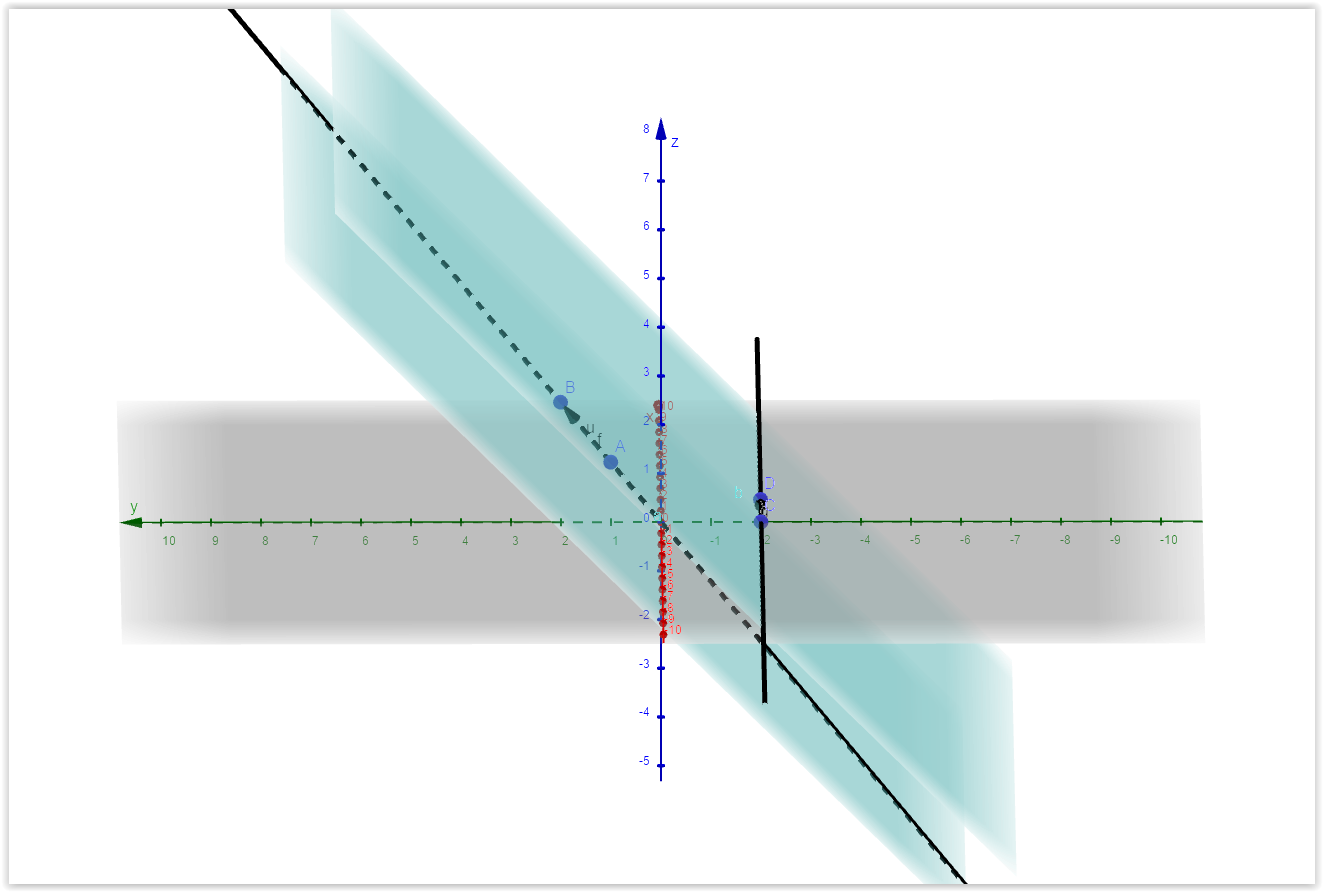
\includegraphics[width=0.5\textwidth]{Abstand_Geraden.png}
		  \caption{Abstand zweier Geraden $\R^3$}
		  \label{fig:abstand_geraden}
	  \end{figure}
	  Zur Bestimmung kann man den Abstandes vom Punkt $a$ (oder jeder andere Punkt auf $g_1$ zur Ebene $E_2$ bestimmen. Hierzu wird die hessesche Normalform von $E_2$ gebildet und $a$ eingesetzt.
\newpage

\section{Logik und Beweise}
  \subsection{Wahrheitswerte}
  \begin{table}[!htpb]
    \caption{Wahrheitswerte}
    \label{wahrheitswerte}
	  \begin{tabular}{|c|c|c|c|c|c|c|c|} \noalign{\hrule height 1.5pt}
		  $w(A$) & $w(B)$ & $\;$ & $w(\neg A)$ & $w(A \land B)$ & $w(A\lor B)$ & $w(A \Rightarrow B$ & $w(A \Leftrightarrow B$ \\ \noalign{\hrule height 1.5pt}
		  $1$  & $1$ & $\;$ & $0$ & $1$ & $1$ & $1$ & $1$\\ \hline
		  $1$  & $0$ & $\;$ & $0$ & $0$ & $1$ & $0$ & $0$\\ \hline
		  $0$  & $1$ & $\;$ & $1$ & $0$ & $1$ & $1$ & $0$\\ \hline
		  $0$  & $0$ & $\;$ & $1$ & $0$ & $0$ & $1$ & $1$\\ \noalign{\hrule height 1.5pt}
	  \end{tabular}
  \end{table}
  \begin{bem}
    Wenn $A \Rightarrow B$ wahr ist, dann heißt $A$ hinreichend für $B$ und $B$ heißt notwendig für $A$.
  \end{bem}
  \subsubsection{Tautologien}
  Tautologien sind Aussagen die immer wahr sind.
  \begin{itemize}
    \item $(A \Rightarrow B) \Leftrightarrow (\neg B \Rightarrow \neg A$
    \item $(A\Rightarrow B) \Leftrightarrow \neg(\neg B \land \neg A)$
    \item $A \lor \neg A$
    \item $\neg(A \land \neg A)$
    \item $\neg(A \land B) \Leftrightarrow \neg A \lor \neg B$ (De Morgansche Regel)
    \item $\neg(A \lor B) = \neg A \land \neg B$ (De Morgansche Regel)
    \item $(A \Rightarrow B) \land (B\Rightarrow C) \Rightarrow (A \Rightarrow C)$
    \item $(A \land (B\lor C)) \Leftrightarrow ((A \land B) \lor (A\land C))$ (Distributivgesetz)
    \item $(A\lor (B\land C)) \Leftrightarrow ((A \lor B) \land (A \lor C))$ (Distributivgesetz)
  \end{itemize} 
  
  \subsubsection{Umformungen}
  \begin{table}[H]
    \caption{Umformungen}
    \label{umformungen}
	  \begin{tabular}{|p{4cm}|p{10cm}|} \noalign{\hrule height 1.5pt}
      \textbf{Form der Negation} & \textbf{umgeformte Aussage} \\ \noalign{\hrule height 1.5pt}
      $\neg(\neg A)$ & $A$ \\ \hline
      $\neg(A \land B)$ & $(\neg A) \lor (\neg B)$ (De Morgansche Regel) \\ \hline
      $\neg(A \lor B)$ & $(\neg A)  \land (\neg B)$ (De Morgansche Regel) \\ \hline
      $\neg(A \Rightarrow B)$ & $A \land (\neg B)$ da $(A \Rightarrow B) \Leftrightarrow \neg A \lor \neg B$ \\ \hline
      $\neg(A \Leftrightarrow)$ & $A  \Leftrightarrow (\neg B)$\\ \hline
      $\neg (\forall x \in M: A(x))$ & $\exists x \in M: \neg A(x)$\\ \hline
      $\neg (\exists x \in M: A(x))$ & $\forall x \in M: \neg A(x)$\\ \noalign{\hrule height 1.5pt}
    \end{tabular}
  \end{table}
  \subsection{Vollständige Induktion}
    \subsubsection{Vorgehen}
    \begin{flalign*}
      &\textbf{Schritt 1: } \text{Induktionsannahme (also was zu zeigen ist)}&
    \end{flalign*}
    \vspace{-0.5cm}
    \begin{flalign*}
      &\textbf{Schritt 2: } \text{Induktionsanfang (meistens $n=1$, ist aber frei wählbar}& \\
    \end{flalign*}
    \vspace{-1cm}
    \begin{flalign*}
      &\textbf{Schritt 3: } \text{Induktionsvorraussetzung (eher optional)}&\\
    \end{flalign*}
    \vspace{-1cm}
    \begin{flalign*}
      &\textbf{Schritt 4: } \text{Induktionsbehauptung}&\\
      &\text{(die Behauptung, dass es für alle n gilt. Bei Summen hier in der Regel $n+1$ einfügen)}&\\
    \end{flalign*}
    \vspace{-1cm}
    \begin{flalign*}
      &\textbf{Schritt 5: } \text{Induktionsschritt (der eigentliche Beweis))}&\\
    \end{flalign*}
    \subsubsection{Beispiel 1}
    \begin{flalign*}
      &\underline{Induktionsannahme:}&\\ 
      &\qquad \qquad z.Z.:\; \forall n \in \N: 11^n - 4^n \text{ ist ein Vielfaches von 7}& \\
    \end{flalign*}
    \vspace{-1.7cm}
    \begin{flalign*}
      &\underline{Induktionsanfang:}&\\
      & n = 1:&\\
      & \; &11^1 - 4^1 &\overset{!}{=} x \cdot 7 \quad , x \in \N && \; &&\\
      &\; &11-4 &= 7 = x \cdot 7&&\; &&\\
      &\; &x &= 1 \checkmark &&\; &&\\
    \end{flalign*}
    \vspace{-1.7cm}
    \begin{flalign*}
      &\underline{Induktionsbehauptung:}&\\
      &\qquad \qquad 11^{n+1}-4^{n+1} = a\cdot 7  \quad , a \in \N \\
    \end{flalign*}
    \vspace{-1.7cm}
    \begin{flalign*}
    &\underline{Induktionsschluss:}&\\
    &\;& &11^{n+1}-4^{n+1} = 11^n \cdot 11-4^n \cdot 4 && \;&&\\
    &\;& &= 11^n (7+4)-4^n \cdot 4  && \;&&\\
    &\;& &= 7 \cdot 11^n + 4 \cdot 11^n + 4 \cdot 4^n  && \;&&\\
    &\;& &= \underbrace{7 \cdot 11^n}_{=(*)} + \underbrace{4(11^n - 4^n)}_{=(**)} && \;&&\\
    \end{flalign*}
    $(*)$ ist duch $7$ teilbar da $7$ ein Faktor ist, $(**)$ ist ebenfalls durch $7$ teilbar, da $(**)$ ein Vielfaches der Induktionsannahme ist, also gilt:
    \begin{flalign*}
    &\;& &7 \cdot 11^n + 4(11^n - 4^n) = b \cdot 7 \quad, b \in \R && \;&&\\
    &\;& &\Rightarrow b = 11^n + \frac{4 \cdot x\cdot 7}{7} = 11^n + 4 \cdot x&& \;&&\\
    \end{flalign*}
    Somit ist $b \cdot 7$ ein Vielfaches von $7$ was zu zeigen war.
  \subsection{Binomialkoeffizienten}
  \begin{satz}
    Es gibt $n! = 1 \cdot 2 \cdot 3 \cdot ...< \cdot (n-1) \cdot n$ Permutationen des n-Tupels $(1,...,n)$. 
  \end{satz}
  \begin{bem}
    Bezeichnung: $n!$ heißt $n$ Fakultät.
  \end{bem}
  Die Verallgemeinerung der binomischen Formel ist gegeben durch:
  \begin{equation}
    (a+b)^n = \sum_{k=0}^n \binom{n}{k} a^k \;0 b^{n-k}
  \end{equation}
  wobei 
  \begin{equation}
    \binom{n}{k} = \frac{n!}{(n-k)!k!}
  \end{equation}
  Binomialkoeffizient heißt und $0! = 1$ gilt.
  \begin{align}
    \begin{array}{c c c c c c c c c c c c}
      \; & \; &  \; & \; & \; &  1 & \; & \; & \; & \; & \;\\
      \; & \; &  \; & \; & 1  & \; &  1 & \; & \; & \; & \;\\
      \; & \; &  \; & 1  & \; & 2  & \; & 1  & \; & \; & \;\\
      \; & \; &  1  & \; & 3  & \; & 3  & \; & 1  & \; & \;\\
      \; & 1  &  \; & 4  & \; &  6 & \; & 4  & \; & 1  & \;\\
      1  & \; &  5  & \; & 10 & \; & 10 & \; & 5  & \; & 1 \\
      \; & \; &  \; & \; & \; &\vdots& \; & \; & \; & \; & \;\\
    \end{array}
    \begin{array}{c}
      \colBlue{(a+b)} \\
      \colBlue{(a+b)^2} \\
      \colBlue{(a+b)^3} \\
      \colBlue{(a+b)^4} \\
      \colBlue{(a+b)^5} \\
    \end{array}
  \end{align}
  bzw.
  \begin{align}
    \begin{array}{c c c c c c c c c c c}
      \; & \; &  \; & \; & \; &  \binom{0}{0} & \; & \; & \; & \; & \;\\
      \; & \; &  \; & \; & \binom{1}{0}  & \; &  \binom{1}{1} & \; & \; & \; & \;\\
      \; & \; &  \; & \binom{2}{0}  & \; & \binom{2}{1}  & \; & \binom{2}{2}  & \; & \; & \;\\
      \; & \; &  \binom{3}{0}  & \; & \binom{3}{1}  & \; & \binom{3}{2}  & \; & \binom{3}{3}  & \; & \;\\
      \; & \binom{4}{0}  &  \; & \binom{4}{1}  & \; &  \binom{4}{2} & \; & \binom{4}{3}  & \; & \binom{4}{4}  & \;\\
      \binom{5}{0}  & \; &  \binom{5}{1}  & \; & \binom{5}{2} & \; & \binom{5}{3} & \; & \binom{5}{4}  & \; & \binom{5}{5} \\
      \; & \; &  \; & \; & \; &\vdots& \; & \; & \; & \; & \;\\
    \end{array}
  \end{align}
  \newpage
  
\section{Mengen, Relationen und Abbildungen}
  \begin{definition}
    Mengen sind Ansammlungen von Elementen.
  \end{definition}
  \subsection{Arten von Mengen}
	  \begin{figure}[htbp] 
		  \centering
		  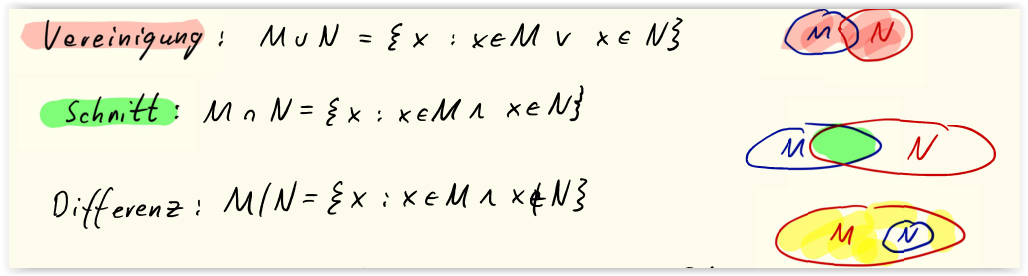
\includegraphics[width=0.9\textwidth]{mengen_arten.png}
		  \caption{Arten von Mengen\protect\cite{HM12}}
		  \label{fig:mengen_arten}
		\end{figure}
	  \begin{definition}
	    Ist $N \subset M$ dann heißt $N^c = M/N$ das Komplement von $N$. $M$ und $N$ heißen disjunkt, falls $M \cap N = \mathcal{O}$, wobei $\mathcal{O} = \lbrace \rbrace$ die leere Menge ist.
	  \end{definition}
	  \begin{definition}
	    Kartesisches Produkt: $M \times N = \lbrace (a,b): a \in M \land b \in N\rbrace$
	  \end{definition}
	  \begin{definition}
	    Potenzmenge: $P(M) = \lbrace X:X\subset M\rbrace$
	  \end{definition}
	  \subsubsection{Abkürzungen}
	  \begin{itemize}
	    \item $\bigcup\limits_{k = 1}^n A_k = A_1 \cup ... \cup A_n$
	    \item $\bigcap\limits_{k=1}^n A_k = A_1 \cap ... \cap A_n$
	    \item $\prod\limits_{k=1}^n A_k = A_1 \times ... \times A_n = \lbrace \underbrace{(a_1, ..., a_n)}_{n-Tupel}:\forall k: a_k \in A_k \rbrace$
	  \end{itemize}
	\subsection{Relationen}
	\begin{definition}
	  Relationen setzen Elemente zweier Mengen in Verbindung. Eine Relatiopn ist eine Teilmenge $R\subset M \times N$ mit $M$ und $N$ als Mengen. Man schreibt:
	  \begin{equation*}
	    xRy \text{ genau dann wenn } (x,y) \in R\subset M\times N
	  \end{equation*}
	  Jede Funktion $f \rightarrow f(x)$ ist eine Relation $R=\lbrace (x, f(x)): x\in \R \rbrace \subset \R \times \R$.
	\end{definition}
	\subsubsection{Äquivalenzrelationen}
	  Eigenschaften:
	  \begin{itemize}
	    \item $aRa$, d.h. $(a,a) \in R$ \colBlue{(Reflexivität)}
	    \item $aRb \Leftrightarrow bRa$, d.h. mit $(a,b)\in R$ ist auch $(b,a) \in R$ \colBlue{(Symmetrie)}
	    \item $aRb \land bRc \Rightarrow aRc$, d.h. mit $(a,b) \in R$ und $(b,c) \in R$ ist auch $(a,c) \in R$ \colBlue{(Transitivität)}
	  \end{itemize}
	  \begin{satz}
	    Ist $R$ eine Äquivalenzrelation, d.h. eine Relation mit obigen Eigenschaften, so zerfällt die Menge $M$ in disjunkte Teilmengen. \newline
	    Beispiel:
	    \begin{align*}
	      M &= \lbrace 1,2,3,4\rbrace \\
	      R &= \lbrace(1,3),(3,1),(1,1),(3,3),(2,4),(4,2),(2,2),(4,4)\rbrace\\
	      &\text{$R$ zerlegt $M$ in zwei Klassen (Teilmengen:}\\
	      \lbrace 2,4\rbrace &= [2]_R = [4]_R\\
	      \lbrace 1,3\rbrace &= \underbrace{[1]_R = [3]_R}_{\text{\parbox{2cm}{\centering% 
Repräsentanten \\[-1ex]der Klasse}}}
	    \end{align*}
	    bzw. allgemein: Äquivalenzklasse zu einem Element $a$ bezüglioch einer Äquivalenzrelation $R$
	    \begin{equation*}
	      [a]_R = \lbrace b \in M : aRb\rbrace
	    \end{equation*}
	    Die Menge aller Äquivalenzklassen ist: $M/_R = \lbrace[a]_R: a\in M\rbrace$. Es gilt entweder $[a]_R = [b]_R$ oder $[a]_R \cap [b]_R = \mathcal{O}$.
	  \end{satz}
	  \begin{bem}
	    Es wird häufig anstatt $R$ das Zeichen $\sim$ verwendet.
	  \end{bem}
	\subsubsection{Ordnungsrelationen}
	\begin{definition}
	  Eine Halbordnung $R\subset M \times M$ auf einer Menge $M$ erfüllt
	  \begin{itemize}
	    \item[(i)]   $xRx$
	    \item[(ii)]  $xRy \land yRx \Rightarrow y=x$
	    \item[(iii)] $xRy \land <Rz \Rightarrow xRz$ \colBlue{(Transitivität)}
	  \end{itemize}
	\end{definition}
	\begin{definition}
	  Ordnungsaxiome im $\R$
	  \begin{itemize}
	    \item[(i)]   $x \leq x$
	    \item[(ii)]  $x \leq y \land y \leq x \Rightarrow y = x$
	    \item[(iii)] $x \leq y \land y \leq z \Rightarrow x \leq z$
	    \item[(iv)] $x \leq y \lor y \leq x$ \colBlue{(Totalordnung)}
	    \item[(v)] $x \Rightarrow x+z \leq y+z$ \colBlue{(Zusammenhang mit Addition)}
	    \item[(vi)] $x\leq y \land z \geq 0 \Rightarrow x \cdot z \leq y \cdot z$ \colBlue{(Zusammenhang mit Multiplikation)}
	  \end{itemize}
	\end{definition}
	\begin{definition}
		Zu $a \in \R$ heißt
		\begin{align}
		  |a|:= 
		  \begin{cases} 
		    &a\quad ,\;falls\;a\geq 0 \\ -&a\quad ,\;falls \; a < 0 
		  \end{cases}
		\end{align}
		der Betrag von $a$.
	\end{definition}
	\subsection{Maximum, Minimum, Supremum, Infimum}
	Im Folgenden sei $M$ eine Teilmenge von $\R$.
	\begin{definition}
	  $x \in \R$ heißt eine obere Schranke von $M$, falls $y \leq x$ für alle $y \in M$ gilt. 
	\end{definition}
	\begin{definition}
	  $x \in \R$ heißt eine untere Schranke von $M$, falls $y \geq x$ für alle $y \in M$ gilt. 
	\end{definition}
	\begin{definition}
	  $M$ heißt beschränkt, falls $M$ nach oben und unten beschränkt ist, d.h. eine obere und eine untere Schranke existieren.
	\end{definition}
	\begin{definition}
	  $s = \sup M \in \R$ heißt das Supremum von $M$ und ist die kleinste obere Schranke, d.h. falls $s$ eine obere Schranke von $M$ ist und ferner jede andere obere Schranke $x$ von $M$ die Ungleichung $x\geq s$ erfüllt.
	\end{definition}
	\begin{definition}$\;$\newline
    \vspace{-0.7cm}
	  \begin{itemize}
	    \item[] Infimum: $\inf M \in \R$ ist die größte untere Schranke
	    \item[] Maximum: $s = \max M \in \R$ heißt das Maximum von $M$, falls $s \in M$ und für alle $x \in M$ gilt: $x\leq s$.
	    \item[] Minimum: $s = \min M \in \R$ heißt das Minimum von $M$, falls $s \in M$ und für alle $x \in M$ gilt: $s \leq x$.
	  \end{itemize}
	\end{definition}
	\begin{bem}
	  Für jede endliche Menge existiert das Maximum und Minimum.
	\end{bem}
	\begin{satz}
	  Jede nicht leere, nach oben beschränkte Menge $M \subset \R$ besitzt ein Supremum. (Analog jede nach unten beschränkte Menge ein Infimum)
	\end{satz}
	\begin{bem}
	  \begin{align}
	    \sup(T) \in T &\Rightarrow \sup(T) = \max(T) \\
	    \inf(T) \in T &\Rightarrow \inf(T) = \min(T)
	  \end{align}
	\end{bem}
	\subsection{Abbildungen}
	Abbildungen sind spezielle Relationen. Eine Abbildung $f$ von einer Menge $M$ in eine Menge $N$ ist eine Vorschrift, die jedem $x \in M$ genau ein $y \in N$ zuordnet. $M$ heißt der Definitionsbereich und $N$ heißt der Bildbereich. 
	\begin{definition}
	  $f: M\rightarrow N$ heißt surjektiv, falls die Gleichung $f(x) = y$ mindestens eine Lösung besitzt und zwar für alle $y \in N$.\newline
	  $f:M\rightarrow N$ heißt injektiv, falls für alle $x_1, x_2 \in M: f(x_1) = f(x_2) \Rightarrow x_1 = x_2$.\newline
	  $f$ heißt bijektiv, falls $f$ sowohl injektiv, als auch surjektiv ist.
	\end{definition}
	\subsection{Unendlichkeit}
	\begin{definition}
	  Eine Menge $M$ heißt endlich, falls es ein $n \in N$ und eine bijektive Abbildung $\Phi: \lbrace 1,...,n\rbrace \rightarrow M$ gibt. Eine Menge $M$ heißt abzählbar, falls es eine bijektive Abbildung $\Phi: \N \rightarrow M$ gibt. Sonst heißt die Menge überabzählbar.
	\end{definition}
	\begin{satz}
	  Die Menge der rationalen Zahlen $\Q$ ist abzählbar.
	\end{satz}
	\begin{satz}
	  Die reelen Zahlen sind überabzählbar.
	\end{satz}
	
	\subsection{Elementare realwertige Funktionen}
	  \subsubsection{Algebraische Funktionen}
	  Durch arithmetische Operationen aufgebaut (+,-,$\cdot$,$\backslash$), z.B.: \newline $f(x) = x^2 + 5x$, $f(x) = \sqrt[3]{x}$
    \subsubsubsection{Polynome (+,-,$\cdot$)}
    \begin{equation}
      y = f(x) = a_n x^n + a_{n-1} x^{n-1} + ... + a_0,\quad a_j \in \R
    \end{equation}  
		\vspace{-0.7cm}  	  
	  \begin{figure}[H] 
		\centering
		\begin{minipage}{.5\textwidth}
		  \centering
		  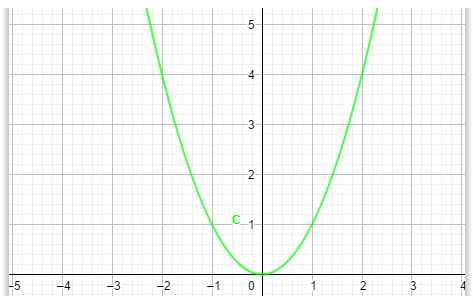
\includegraphics[width=0.7\linewidth]{funktionen_quadratisch.png}
		  \caption{$y = x^2\quad (vgl.\; x^4, x^6, ...)$}
		  \label{fig:funkt_quadr}
		\end{minipage}%
		\begin{minipage}{.5\textwidth}
		  \centering
		  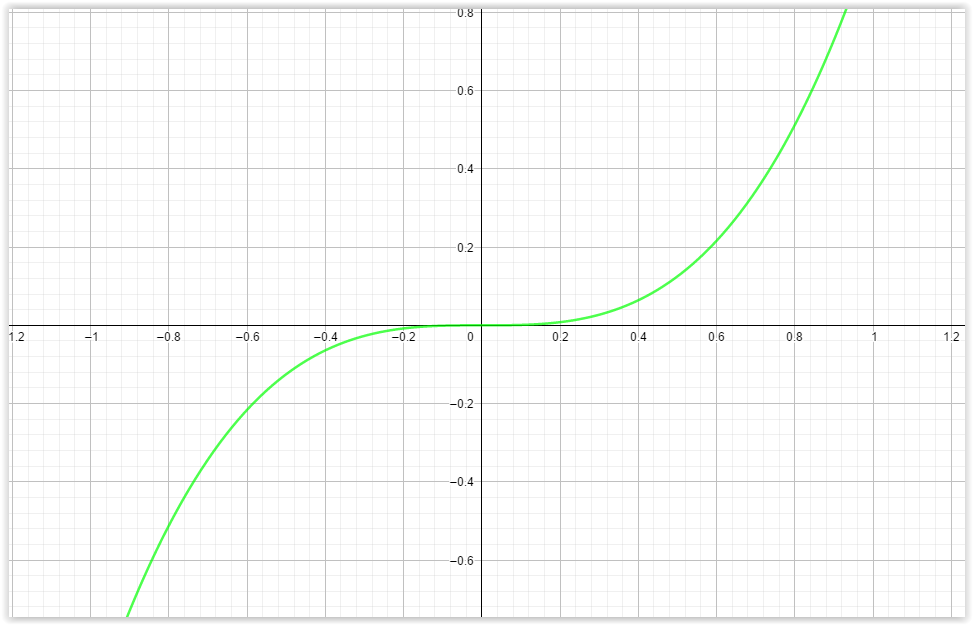
\includegraphics[width=0.7\linewidth]{funktionen_kubisch.png}
		  \caption{$y = x^3 \quad (vgl.\;x^5, x^7, ...)$}
		  \label{fig:funkt_kub}
		\end{minipage}
		\end{figure}
		\vspace{-0.5cm}
		\begin{figure}[H]
		  \centering
		  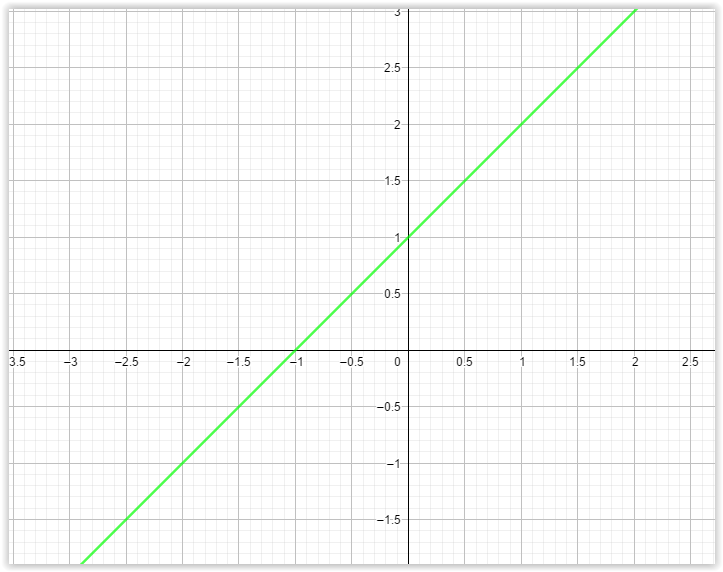
\includegraphics[width=0.3\linewidth]{funktionen_linear.png}
		  \caption{$y = ax+b$}
		  \label{fig:funkt_lin}
		\end{figure}
		
		\vspace{-0.5cm}
		\newpage
		\subsubsubsection{Rationale Funktionen (+,-,$\cdot$, $\backslash$)}
		\begin{equation}
		  y = f(x) = \frac{p(x)}{q(x)} \qquad \text{mit } p,q \text{ sind Polynome}
		\end{equation}
		\begin{figure}[H] 
		\centering
		\begin{minipage}{.5\textwidth}
		  \centering
		  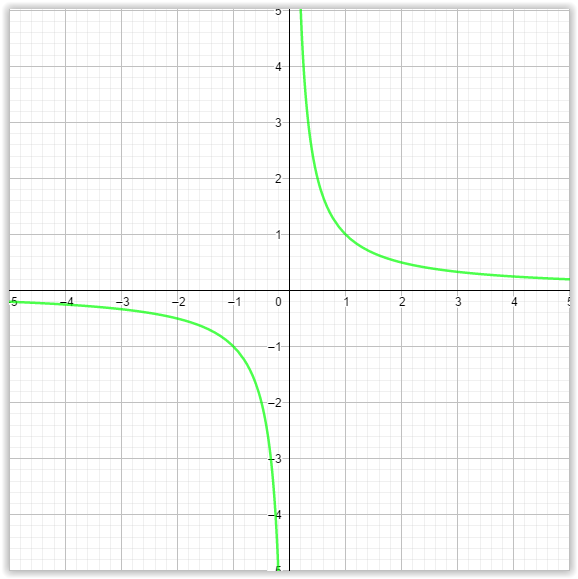
\includegraphics[width=0.6\linewidth]{funktionen_pole_1.png}
		  \caption{$y = \frac{1}{x}$}
		  \label{fig:funkt_pole_1}
		\end{minipage}%
		\begin{minipage}{.5\textwidth}
		  \centering
		  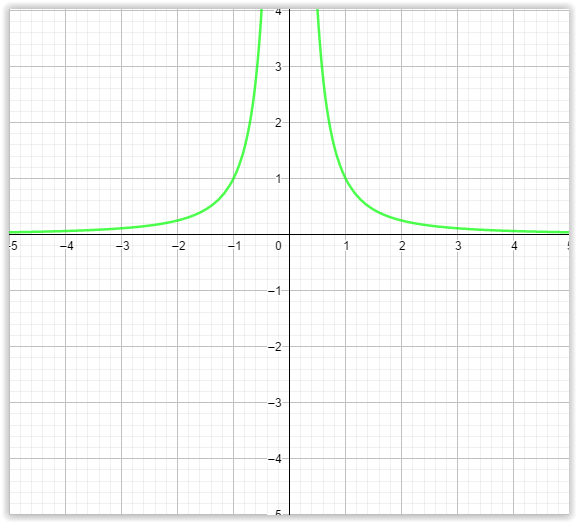
\includegraphics[width=0.65\linewidth]{funktionen_pole_2.png}
		  \caption{$y = \frac{1}{x^2}$}
		  \label{fig:funkt_pole_2}
		\end{minipage}
		\end{figure}
		
		\subsubsubsection{n-te Wurzel}
		\begin{equation}
		  y = f(x) = \sqrt[n]{x}
		\end{equation}
		\begin{figure}[H] 
		\centering
		\begin{minipage}{.5\textwidth}
		  \centering
		  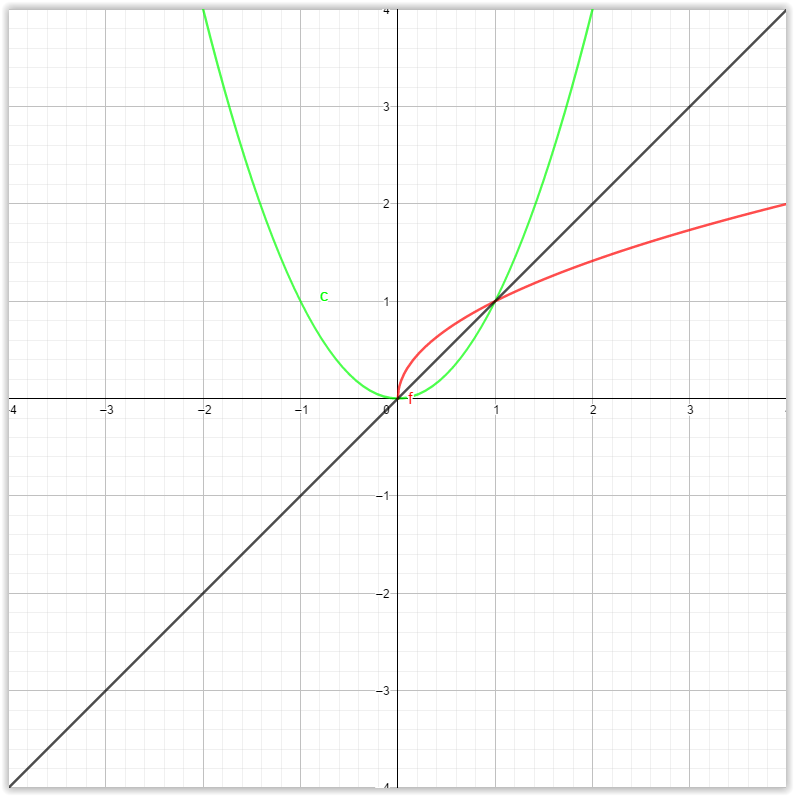
\includegraphics[width=0.6\linewidth]{funktionen_wurzel_2.png}
		  \caption{Quadratwurzel}
		  \label{fig:funkt_root_1}
		\end{minipage}%
		\begin{minipage}{.5\textwidth}
		  \centering
		  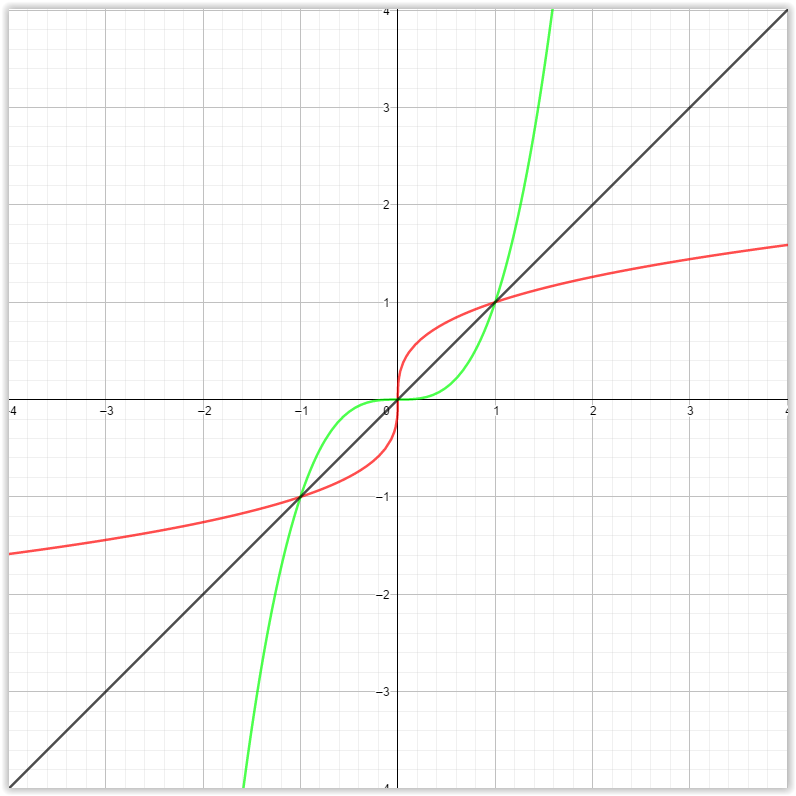
\includegraphics[width=0.6\linewidth]{funktionen_wurzel_3.png}
		  \caption{Kubische Wurzel}
		  \label{fig:funkt_root_2}
		\end{minipage}
		\end{figure}
		Wie man an den Graphiken erkennt ist die Wurzel gerade die Spiegelung an der Ursprungsgeraden des korrelierenden Polynoms. 
		
		\subsubsection{Transzendentale Funktionen}
		\subsubsubsection{Exponentialfunktionen}
		\begin{equation}
		  y =? f(x) = e^x \qquad, e = 2,7182...
		\end{equation}
		Streng monoton wachsende Funktion. Es gilt:
		\begin{equation}
		  \lim_{x\rightarrow \infty} e^x = \infty \qquad \lim_{x\rightarrow -\infty} e^x = 0
		\end{equation}
		
		\subsubsubsection{Unendliche Summen}
		Zum Beispiel Taylorreihen, Potenzreihen
		
		\subsubsubsection{(Natürlicher) Logarithmus}
		\begin{equation}
		  y = f(x) = ln(x)
		\end{equation}
		Bildet das Inverse der e-Funktion. 
		\begin{figure}[H]
		  \centering
		  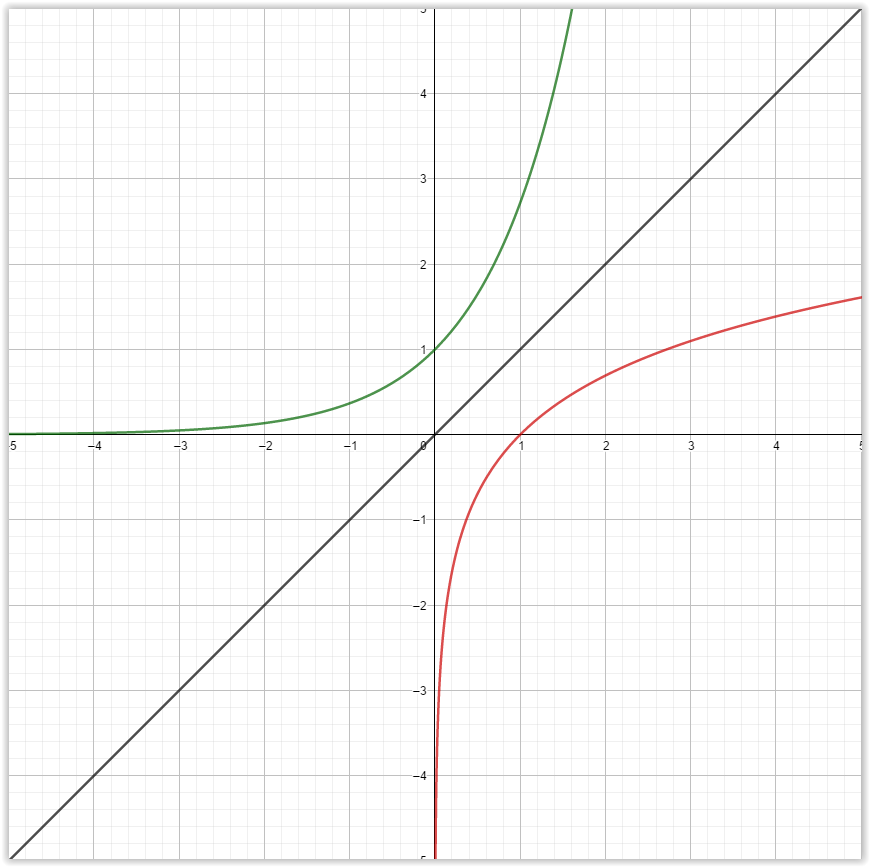
\includegraphics[width=0.35\linewidth]{funktionen_e_ln.png}
		  \caption{Grün: $y = e^x$; Rot: $y = ln(x)$}
		  \label{fig:funkt_e_ln}
		\end{figure}
		Zum Wechsel der Basis können die Logarithmusgesetze angewandt werden:
		\begin{align}
		  h(x) &= a^x = e^{x \cdot ln(x)} \text{, da } ln(a^x) = x\;ln(a) \nonumber \\
		  k(x) &= log_a(x) = \frac{ln(x)}{ln(a)}
		\end{align}
		
		\subsubsubsection{Trigonometrische Funktionen}
		\begin{figure}[H]
		  \centering
		  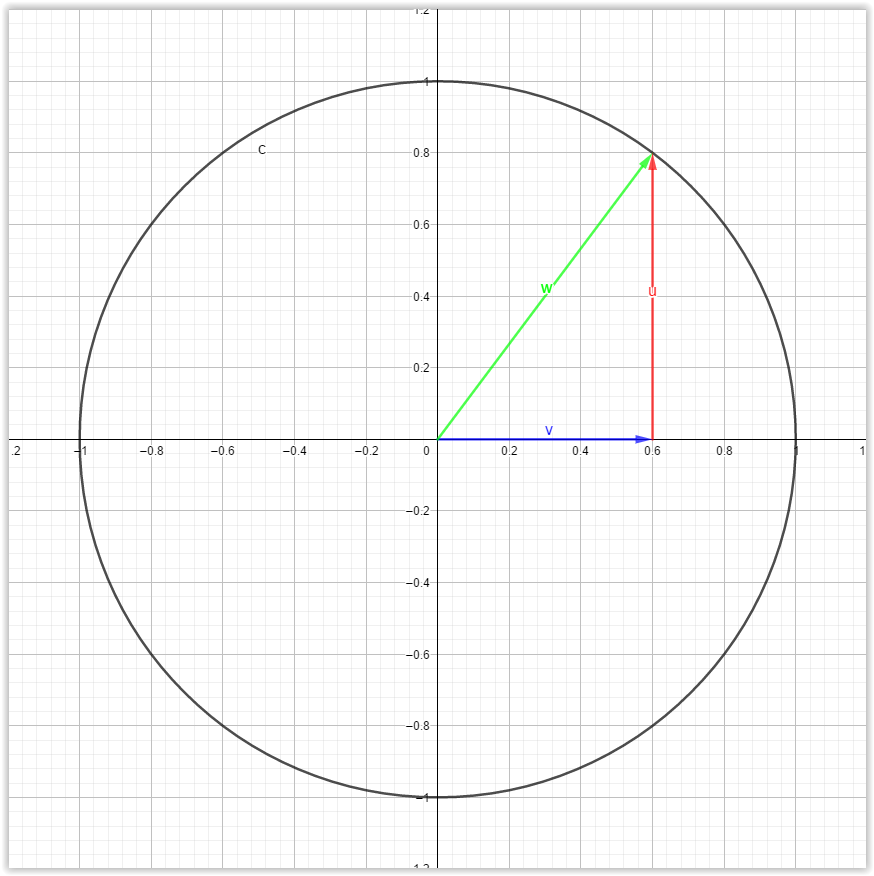
\includegraphics[width=0.35\linewidth]{funktionen_einheitskreis_sin_cos.png}
		  \caption{Grün: $1$; Rot: $sin(x)$; Blau: $cos(x)$}
		  \label{fig:funkt_e_ln}
		\end{figure}
		Aus dem Einheitskreis geht die Identität
		\begin{equation}
		  sin^2(x) + cos^2(x) = 1
		\end{equation}
		direkt hervor.
		\begin{figure}[H] 
		\centering
		\begin{minipage}{.5\textwidth}
		  \centering
		  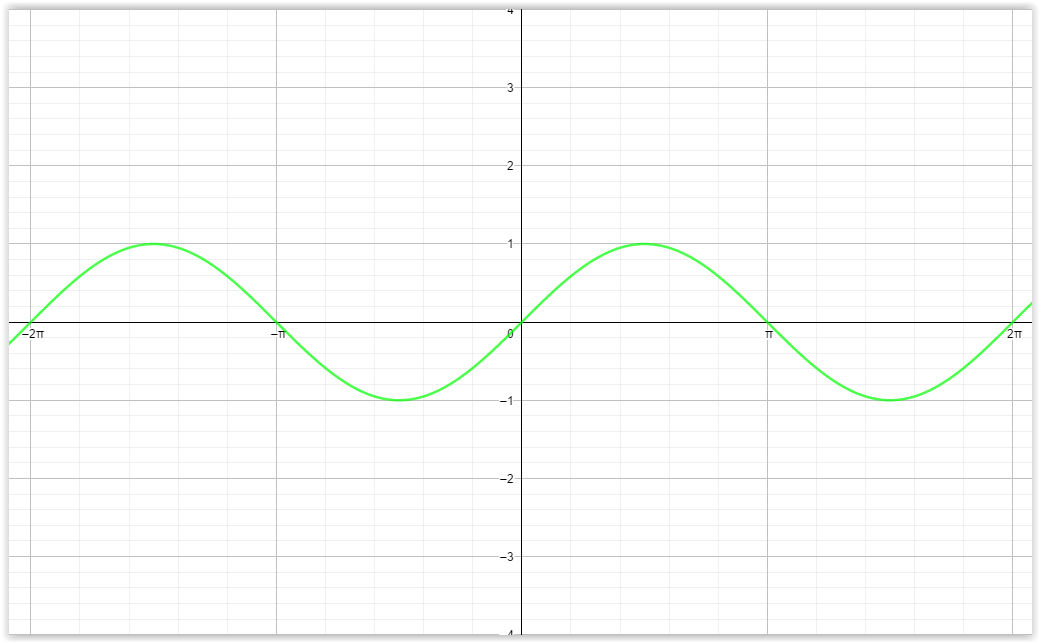
\includegraphics[width=0.9\linewidth]{funktionen_sin.png}
		  \caption{Sinusfunktion}
		  \label{fig:funkt_sin}
		\end{minipage}%
		\begin{minipage}{.5\textwidth}
		  \centering
		  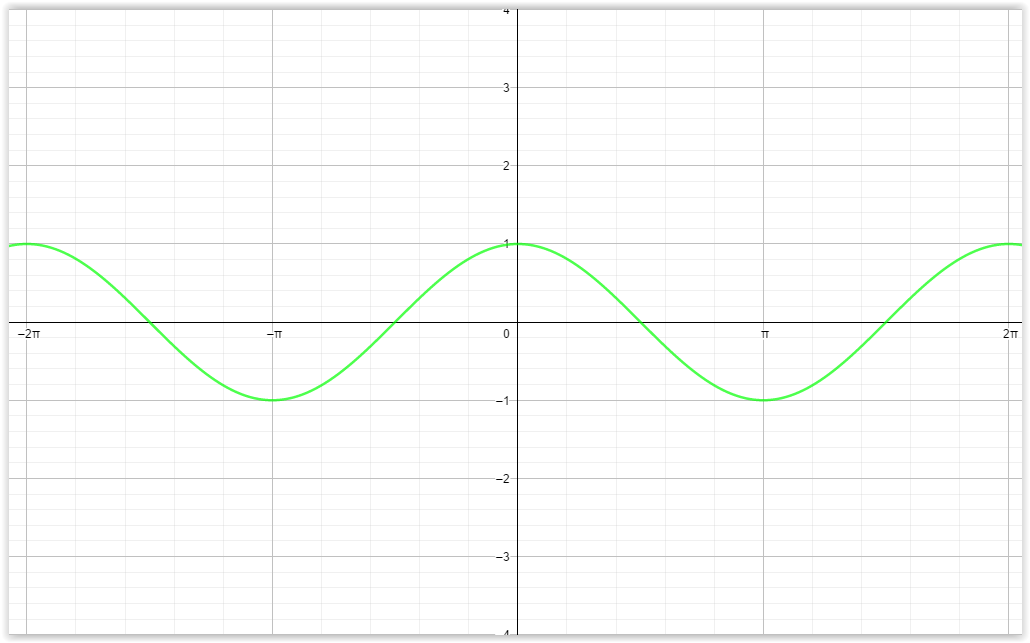
\includegraphics[width=0.9\linewidth]{funktionen_cos.png}
		  \caption{Cosinusfunktion}
		  \label{fig:funkt_cos}
		\end{minipage}
		\end{figure}
		Es gelten folgende Zusammenhänge:\newline
		$\;$\newline
			\begin{tabular}{l | l}
				\tabitem $cos(x) = cos(-x)$ & 
				  \tabitem $e^z = e^{Re\lbrace z \rbrace} \left(cos(Im(z))+isin(Im(z))\right) \quad, z \in \C$\\
				\tabitem $-sin(x) = sin(-x)$ & \tabitem $sin(x) = \frac{1}{2i}\left(e^{ix}-e^{-ix}\right) \quad, x \in \R$\\
				\tabitem $cos(x+2 \pi) = cos(x)$ &  \tabitem $cos(x) = \frac{1}{2}\left(e^{ix}+e^{-ix}\right) \quad, x \in \R$\\
				\tabitem $sin(x+2\pi) = sin(x)$ & $\;$
		\end{tabular} \newline
		$\;$ \newline
		Weiterhin gilt:
		\begin{figure}[H]
		  \centering
		  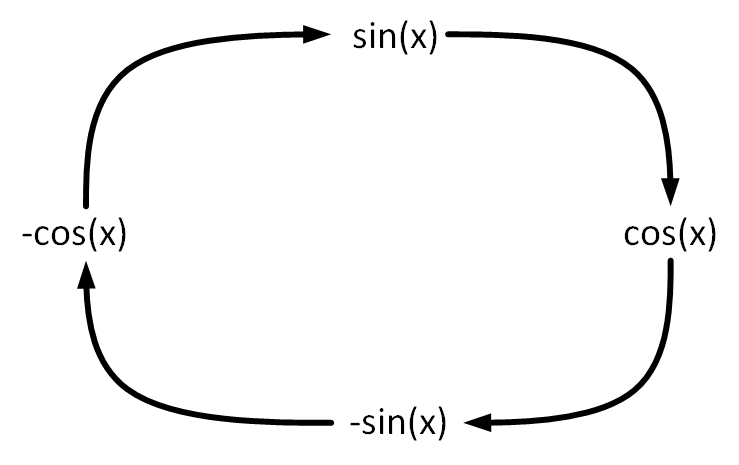
\includegraphics[width=0.35\linewidth]{ableitungskreis.png}
		  \caption{Ableitungsregel}
		  \label{fig:funkt_trigo_abl_1}
		\end{figure}
		\subsubsubsection{Weitere trigonometrische Funktionen}
		\begin{equation}
		  tan(x) = \frac{sin(x)}{cos(x)}, \qquad  csc(x) = \frac{1}{sin(x)}, \qquad  cot(x),\; \dots
		\end{equation}
		\vspace{-0.5cm}
		\begin{figure}[H]
		  \centering
		  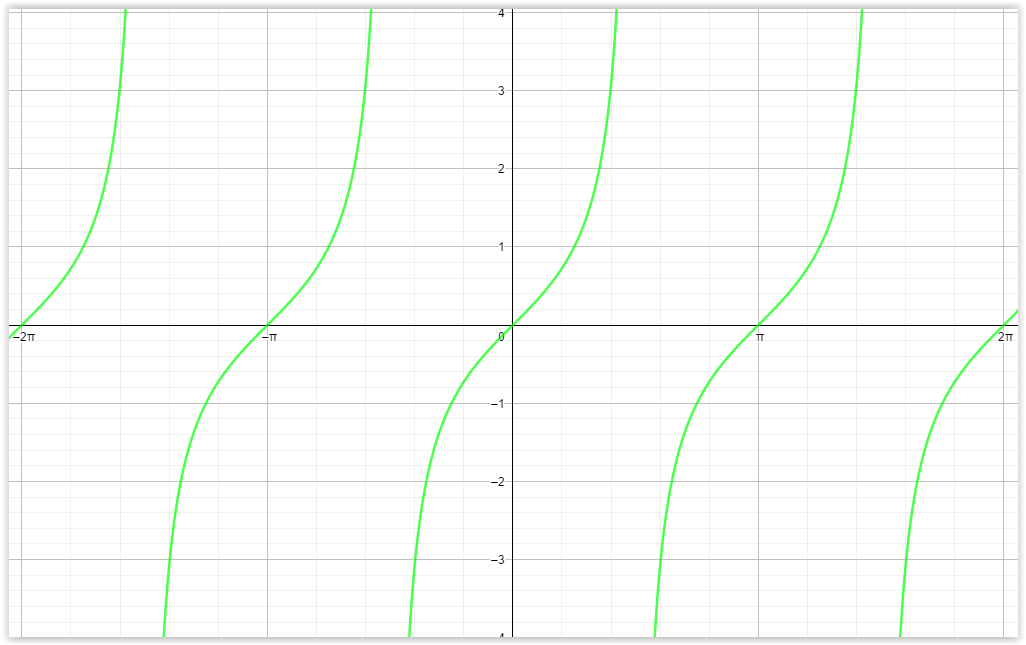
\includegraphics[width=0.5\linewidth]{funktionen_tan.png}
		  \caption{$tan(x)$}
		  \label{fig:funkt_tan}
		\end{figure}
		\subsubsubsection{Hyperbolische Funktionen}
		\begin{align}
		  cosh(x) &= \frac{1}{2}\left( e^x + e^{-x}\right)\nonumber \\
		  sinh(x) &= \frac{1}{2}\left( e^x - e^{-x}\right)\nonumber \\
		  tanh(x) &= \frac{sinh(x)}{cosh(x)}\nonumber \\
		  sech,\;coth&,\; \dots ,\; etc.
		\end{align}
		\vspace{-0.7cm}  	  
	  \begin{figure}[H] 
		\centering
		\begin{minipage}{.5\textwidth}
		  \centering
		  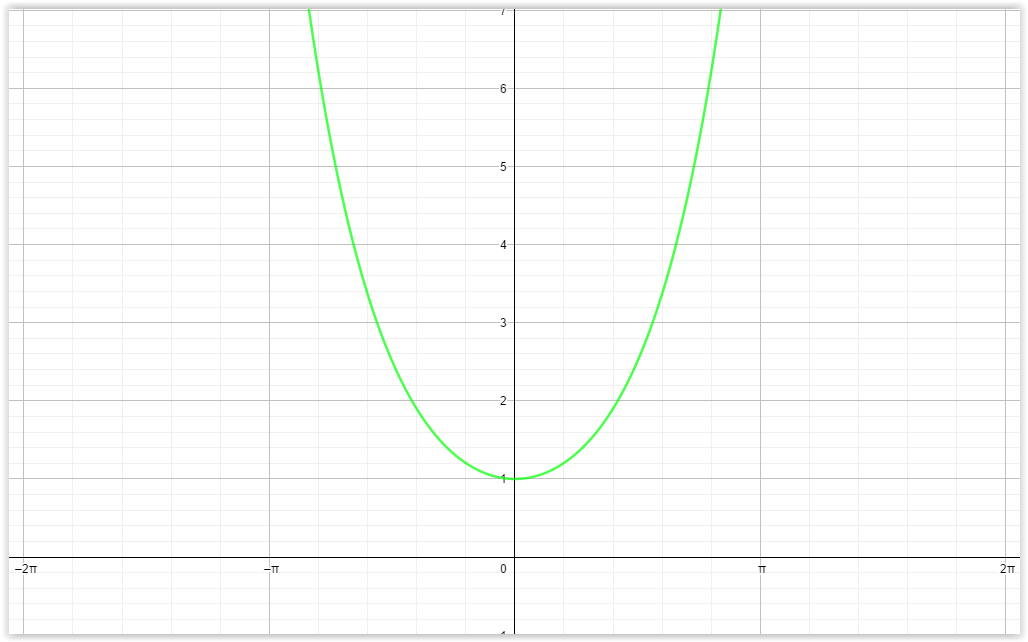
\includegraphics[width=0.8\linewidth]{funktionen_cosh.png}
		  \caption{$y = cosh(x)$}
		  \label{fig:funkt_cosh}
		\end{minipage}%
		\begin{minipage}{.5\textwidth}
		  \centering
		  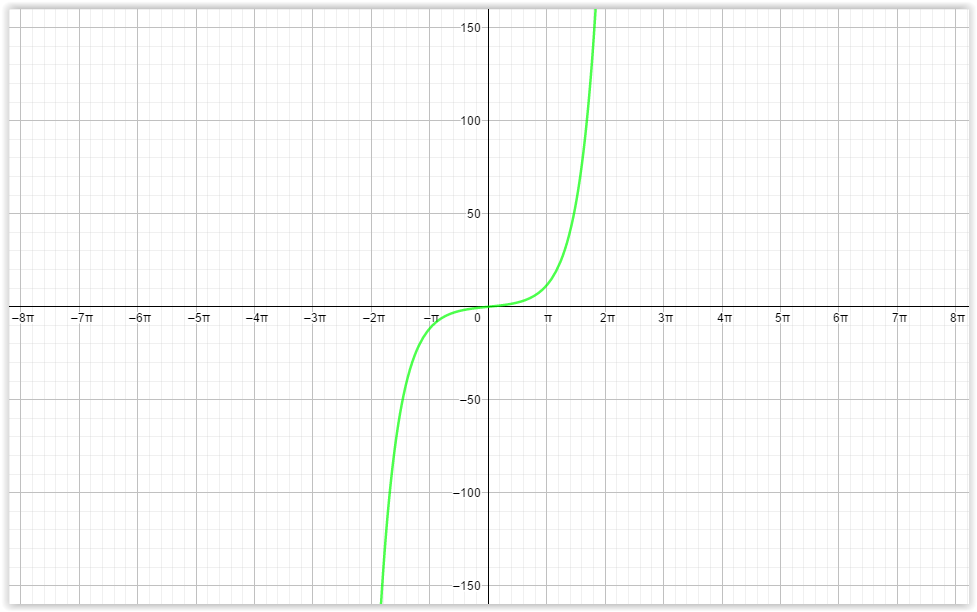
\includegraphics[width=0.8\linewidth]{funktionen_sinh.png}
		  \caption{$y = sinh(x)$}
		  \label{fig:funkt_sinh}
		\end{minipage}
		\end{figure}
		\vspace{-0.5cm}
		\begin{figure}[H]
		  \centering
		  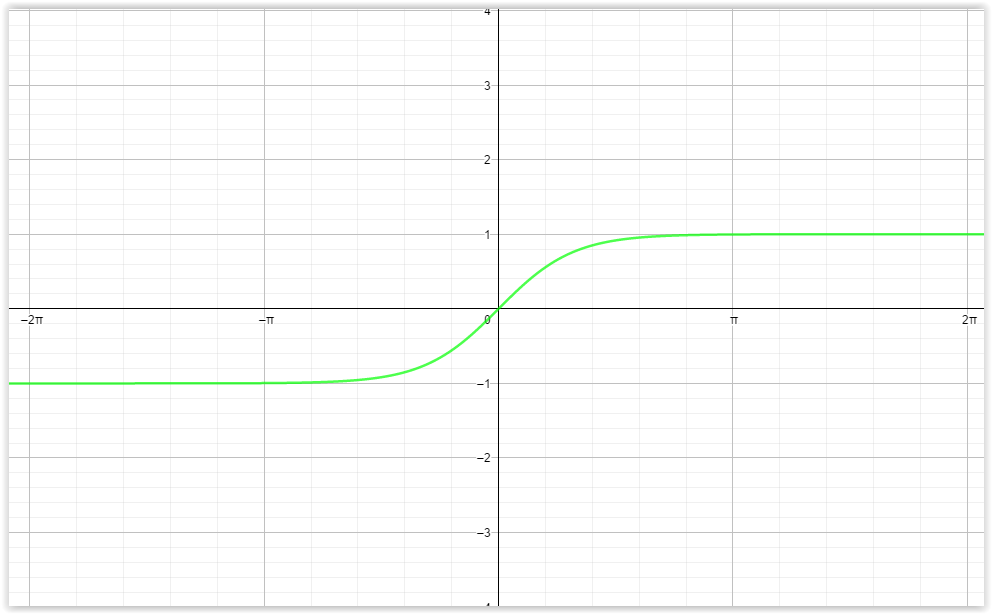
\includegraphics[width=0.4\linewidth]{funktionen_tanh.png}
		  \caption{$y = tanh(x)$}
		  \label{fig:funkt_tanh}
		\end{figure}
		Es gelten folgende Identitäten:
		\begin{align}
		  \big(cosh(x)\big)' &= sinh(x) \\
		  \big(sinh(x)\big)' &= cosh(x) \\
		  cosh^2(x) - sinh^2(x) &= 1 \\
		  cos(z) &= \frac{1}{2}\left(e^{iz}+e^{iz}\right) = cosh(iz) \quad , z \in \C \\
		  sin(z) &= \frac{1}{2i}\left( e^{iz} - e^{iz}\right) = -isinh(/iz) \quad , z \in \C
		\end{align}
\newpage

\section{Konvergente Folgen}
  \begin{definition}
    Eine Folge in einer Menge $M$ ist eine Abbildung $\N \rightarrow M,\; n\rightarrow a_n$. Wir schreiben $(a_n)_{n \in \N}$. Für $n_j \in \N$ mit $1\leq n_1 < n_2 < n_3 < ...$ heißt $(a_{n_j})_{j\in \N}$ eine Teilfolge von $(a_n)_{n \in \N}$.
  \end{definition}
  Beispiele:
  \begin{align*}
    (a_n)_{n \in \N}\; mit\; a_n = \frac{1}{n} \qquad , 1, \frac{1}{2}, \frac{1}{3}, \frac{1}{4},...\\
    Teilfolge\;a_1, a_5, a_8, a_{17},... \qquad  ,1 \frac{1}{5}, \frac{1}{8}, \frac{1}{17}, ...
  \end{align*}
  \subsection{Vergleich expliziter und rekursiver Darstellung}
  \begin{tabular}{l c l}
    $a_n = (-1)^n ,\quad n \in \N$ & $\rightarrow$ & $a_{n+1} = -a_n,\quad a_1 = -1$\\
    $a_n = n! quad n \in \N$ & $\leftarrow$ & $ a_n = n \cdot a_{n-1}, \quad n \geq 2, \quad a_1 = 1$\\
    $\;$ & $\;$ & $a_1 = 1$ \\
    $\;$ & $\;$ & $a_2 = 2\cdot a_1 = 2 \cdot 1$ \\
    $\;$ & $\;$ & $a_3 = 3\cdot a_2 = 3 \cdot 2 \cdot 1$ \\
  \end{tabular}    

  
  \subsection{Definitionen $\varepsilon-N$-Kriterium/Konvergenzkriterium}
  \begin{definition}
    Es sei $(a_n)_{n \in \N}$ eine Folge in $\R$.
    \begin{itemize}
      \item[a)] Eine Folge $(a_n)_{n \in \N}$ heißt beschränkt, falls es ein $C > 0$ gibt, mit $|a_n| \leq C$ für alle $n \in \N$.
      \item[b)] Eine Folge $(a_n)_{n \in \N}$ heißt konvergent mit Grenzwert (Limes) $a$, falls für alle $\varepsilon > 0$ ein $N\in \N$ existiert, so dass für alle $n \in \N$ mit $n \geq N$ gilt: $|a_n - a| < \varepsilon$. Eine nicht kovergente Folge heißt divergent.
      \begin{equation}
        Konvergenzkriterium:\; \forall \varepsilon > 0 \quad \exists N(\varepsilon) \in \N \quad \forall n \geq N(\varepsilon): |a_n -a| < \varepsilon \label{eq:folge_konvergenz}
      \end{equation}
      \item[c)] Die möglichen Grenzwerte von Teilfolgen heißen Häufungspunkte.
    \end{itemize}\label{def:folge_konvergenz}
  \end{definition}
  \begin{figure}[htbp] 
	  \centering
	  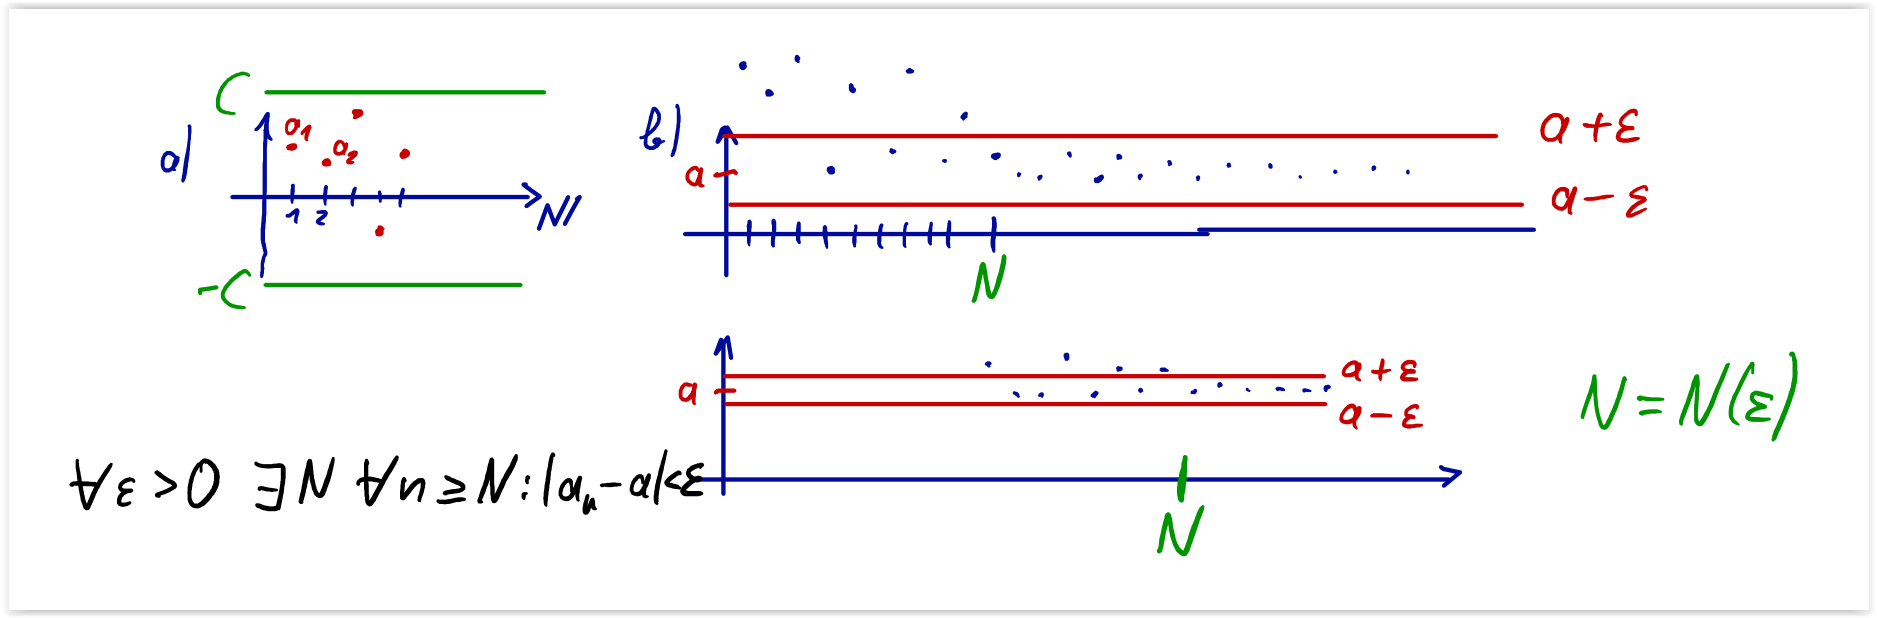
\includegraphics[width=0.9\textwidth]{folge_epsil_krit.png}
	  \caption{Epsilon Kriterium\protect\cite{HM12}}
	  \label{fig:folge_epsilon}
	\end{figure}
  \begin{bem}
    Konvergiert $(a_n)_{n \in \N}$ gegen $a$ schreibt man
    \begin{align}
      &\lim_{n \rightarrow \infty} a_n = a\\
      &bzw. \nonumber \\
      &a_n \underset{n \rightarrow \infty}{\rightarrow} a \nonumber
    \end{align}
  \end{bem}
  \begin{bem}
    Die Schranke $N$ ist i.A. von $\varepsilon$ abhängig. Daher schreibt man $N(\varepsilon)$.
  \end{bem}
  \begin{bem}
    Der Grenzwert einer Folge ist eindeutig.
  \end{bem}
  
  \subsection{Ausdrücke mit Brüchen}
  $(a_n)$ mit $a_n = \frac{P(n)}{Q(n)}$ mit $P,Q$ sind Polynome.
  \begin{align*}
    \textbf{(1)}\quad grad(P) > grad(Q) &\Rightarrow (a_n) \text{ divergiert} \\
    \textbf{(2)}\quad grad(P) < grad(Q) &\Rightarrow (a_n) \text{ konvergiert gegen } 0\\
    \textbf{(3)}\quad grad(P) = grad(Q) &\Rightarrow (a_n) \text{ konvergiert gegen Quotient der Leitkoeffizienten}
  \end{align*}   
  
  \subsection{Dreiecksungleichung}
  \begin{align}
    |x+y| &\leq |x| + |y| \qquad ,\; x,y \in \R \\
    \text{bzw. in umgekehrter Form} \nonumber \\
    \big| |x| - |y| \big| &\leq |x-y|
  \end{align}
  
  \subsection{Beschränktheit}
  \begin{satz}
    Eine konvergente reelle Folge ist beschränkt.
  \end{satz}
  \begin{figure}[H] 
	  \centering
	  
\includegraphics[width=0.3\textwidth]{beschraenkt.jpg}
	  \caption{derp derp derp}
	  \label{fig:folge_epsilon}
	\end{figure}
  
  \subsection{Grenzwertsätze}
  \begin{satz}
    Seien $(a_n)$, $(b_n)$ konvergente Folgen. Dann konvergieren auch die Folgen $\big(|a_n|\big)$, $(a_n + b_n)$ und $(\lambda a_n)$ für $\lambda \in \R$, und es gilt:
    \begin{itemize}
      \item[i) ] ~\\[-28pt]
      \begin{equation}
        \lim|a_n| = |\lim a_n|
      \end{equation}
      \item[ii) ] ~\\[-28pt]
      \begin{equation}
        \lim (a_n \pm b_n) = \lim a_n \pm \lim b_n
      \end{equation}       
      \item[iii) ] ~\\[-28pt]
      \begin{equation}
        lim (\lambda a_n) = \lambda \lim a_n
      \end{equation}
    \end{itemize}
  \end{satz}
  \begin{satz}
    Seien $(a_n)$, $(b_n)$ konvergente Folgen.
    \begin{itemize}
      \item[iv) ] Dann konvergiert auch $(a_n b_n)$ und es gilt\newline
      \begin{equation}
        lim (a_n b_n) = (\lim a_n)(\lim b_n)
      \end{equation}
      \item[v) ] Ist $b_n \neq 0$ für alle $n \in \N$ und $b \neq 0$, so konvergiert auch $\left( \frac{a_n}{b_n} \right)$ mit
      \begin{equation}
        \lim \left( \frac{a_n}{b_n} \right) = \frac{\lim a_n}{\lim b_n}
      \end{equation}
      \item[vi) ] Sei $m \in \N$. Ist $a_n \geq 0$ für alle $n \in \N$, dann konvergiert auch $\big( \sqrt[m]{a_n}\big)$ und es gilt
      \begin{equation}
        \lim \sqrt[m]{a_n} = \sqrt[m]{\lim a_n}
      \end{equation}
    \end{itemize}
  \end{satz}
  \begin{bem}
    Bei rationalen Ausdrücken mit der höchsten Potenz durchkürzen. Beispiel:
    \begin{equation*}
      \frac{n}{n^2+4n+8} = \frac{\frac{1}{n}}{1+\frac{4}{n}+\frac{8}{n^2}} \rightarrow \frac{0}{1}=0
    \end{equation*}
  \end{bem}
  
	  \subsubsection{Beispiele wichtiger Grenzwerte}
	  \begin{itemize}
	    \item[1) ] $\lim \frac{1}{n} = 0$
	    \item[2) ] Sei $q \in \R$ mit $|q| < 1$:\newline
	      $\lim q^n = 0$
	    \item[3) ] Sei $q \in \R$ mit $|q| < 1$ und $p \in \Z$:\newline
	      $\lim n^p q^n = 0$
	    \item[4) ] Sei $a \in \R$:\newline
	      $\lim \frac{a^n}{n!} = 0$
	    \item[5) ] $\;$\newline
	      $\lim\limits_{n \rightarrow \infty} \frac{n^k}{a^n} = 0$
	    \item[6) ] $\;$\newline
	      $\lim\limits_{n \rightarrow \infty} \sqrt[n]{c} = 1$
	    \item[7) ] $\;$\newline
	      $\lim\limits_{n \rightarrow \infty} \sqrt[n]{n} = 1$
	  \end{itemize}
	  
	\subsection{Konvergenzsätze}
	\begin{satz} $\;$\newline
	  \begin{itemize}
	    \item[1) ] Der Grenzwert einer konvergenten Folge ist eindeutig.
	    \item[2) ] Jede konvergente Folge ist beschränkt.
	    \item[3) ] Jede monotone und beschränkte Folge ist konvergent.
	      \begin{itemize}
	        \item[a) ]$(a_n)$ ist monoton wachsend und nach oben beschränkt 
	        \begin{equation*}
	          \Rightarrow \lim\limits_{n \rightarrow \infty} a_n = \sup\limits_{n \in \N} (a_n)
	        \end{equation*}
	        \item[b) ]$(a_n)$ ist monoton fallend und nach unten beschränkt 
	        \begin{equation*}
	          \Rightarrow \lim\limits_{n \rightarrow \infty} a_n = \inf\limits_{n \in \N} (a_n)
	        \end{equation*}
	      \end{itemize}
	  \end{itemize}
  \end{satz}  
  
  \subsection{Monotene Folgen}
  \begin{definition}
    Eine reelle Folge $(a_n)_{n \in \N}$ heißt monoton wachsend, falls $a_n \leq a_{n+1}$ für alle $n \in \N$. Sie heißt streng monoton wachsend, falls $a_n < a_{n+1}$ für alle $n \in \N$. Analog monoton fallend und streng monoton fallend.
  \end{definition}
  \begin{satz}
    Ist die Folge $(a_n)_{n \in \N}$ monoton wachsend und nach oben beschränkt, so konvergiert die Folge und es gilt
    \begin{equation}
      \lim_{n\rightarrow \infty} a_n = \sup \lbrace a_n : n\in \N \rbrace
    \end{equation}
  \end{satz}
  \begin{figure}[htbp] 
	  \centering
	  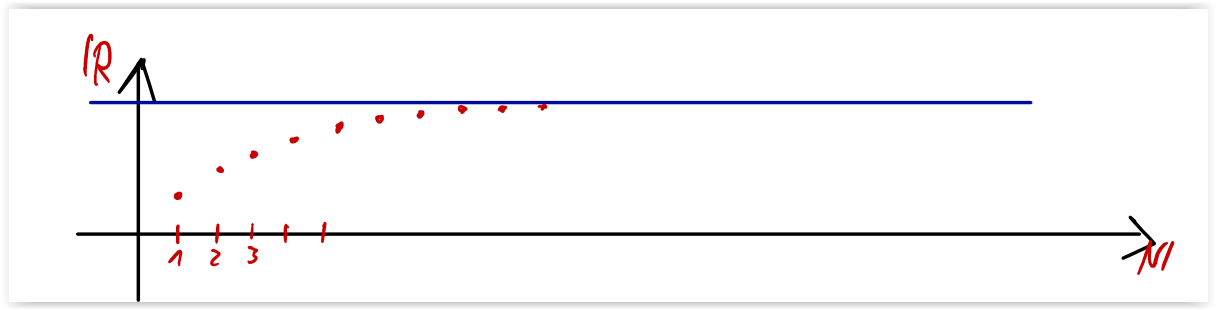
\includegraphics[width=0.9\textwidth]{folge_monoton_beschraenkt.png}
	  \caption{Konvergenz mw u. beschr. Folgen\protect\cite{HM12}}
	  \label{fig:folge_mw_beschr}
	\end{figure}
	
		\subsubsection{Intervallschachtelung}
		Es seien $(a_n)_{n \in \N}$ und $(b_n)_{n \in \N}$ reelle Folgen.
		$(a_n)_{n \in \N}$ sei monoton wachsend und $(b_n)_{n \in \N}$ sei monoton fallend. Es gelte $(a_n)_{n \in \N} \leq (b_n)_{n \in \N}$ für alle $n \in \N$.
    Dann gilt 
    \begin{equation*}
      \lim_{n \rightarrow \infty} a_n,\quad \lim_{n \rightarrow \infty} b_n \quad ex.
    \end{equation*}
    und
    \begin{equation}
      \lim_{n \rightarrow \infty} (b_n - a_n) = 0 \Rightarrow \lim_{n \rightarrow \infty} a_n = \lim_{n \rightarrow \infty} b_n
    \end{equation}
\newpage

\section{Ableitung}
  \subsection{Differenzenquotient/Differentialquotient}
  \begin{definition}
    Die Änderung einer Funktion heißt Differenzenquotient:
    \begin{equation}
      \frac{f(x_n)-f()x_0)}{x_n - x_o}
    \end{equation}
  \end{definition}
  \begin{definition}
    Gegeben sei $f: I\rightarrow \R$ und ein Punkt $x_o \in I$. Die Funktion $f$ heißt differenzierbar in $x_0$, falls der Grenzwert
    \begin{equation}
      \lim_{x\rightarrow x_0} \frac{f(x) - f(x_0)}{x - x_0} = \lim_{h \rightarrow 0} \frac{f(x_0 + h) - f(x_0)}{h}
    \end{equation}
    existiert. Der Grenzwert heißt der Differentialquotient bzw. die Ableitung von $f$ in $x_0$ und wird mit $f'(x_0)$ bzw. $\diff{f}{x}(x_0)$ bezeichnet.
  \end{definition}
  \begin{bem}
    Die Ableitung $f'(x_0)$ gibt die Steigung der Tangente an $f$ in $x_0$ an. Die Tangentengleichung ist:
    \begin{equation}
      l(x) = f(x_0) + f'(x_0)(x-x_0)
    \end{equation}
    Es gilt:
    \begin{align}
      &l(x_0) = f(x_0) + f'(x_0)(x_0 - x_0) = f(x_0) \\
      und\nonumber \\
      &l'(x_0) = f'(x_0)
    \end{align}
    d.h. der Funktionswert und die Ableitung von $f$ und $l$ stimmen in $x_0$ überein.
  \end{bem}
  \subsection{Stetigkeit}
  \begin{definition}
    Eine Funktion $f$ heißt stetig in $x_0$, falls 
    \begin{equation}
      \lim_{x \rightarrow x_0} f(x) = f(x_0)
    \end{equation}
  \end{definition}
  \begin{satz}
    Jede in $x_0$ differenztierbare Funktion ist auch stetig in $x_0$  
  \end{satz}
  \begin{bem}
    Merkregel:\newline
    Stetig: $f$ kann durchgezeichnet werden.\newline
    Diffbar: $f$ hat keinen Knick
  \end{bem}
  Beispiel:\newline
  $f(x) = |x|$ ist in $x_0 = 0$ stetig aber nicht diffbar.
  \begin{bem}
    Bezeichnungen:
    \begin{itemize}
      \item $C^0$: Menge aller stetigen Funktionen
      \item $C^1$: Menge aller diffbaren Funktionen mit $f,f'$ stetig
      \item $C^n$: Menge der n-mal stetig diffbaren Funktionen, d.h. $f, f', \dots, f^{(n)}$
      \item $C^{\infty}$: Menge aller unendlich oft stetig diffbaren Funktionen
    \end{itemize}
  \end{bem}
  \subsection{Wichtige Ableitungen}
  \begin{equation}
    f(x) = x^n \rightarrow f'(x) = nx^{n-1}
  \end{equation}
  \begin{equation}
    f(x) = e^x \Rightarrow f'(x) = e^x
  \end{equation}
  \begin{equation}
    f(x) = ln(x) \Rightarrow f'(x) = \frac{1}{x}
  \end{equation}
  \begin{equation}
    f(x) = arctan(x) \Rightarrow f'(x) = \frac{1}{(tan(y))'}
  \end{equation}
  \begin{equation}
    f(x) = arcsin(x) \Rightarrow f'(x) = \frac{1}{(sin(y))'}
  \end{equation}

  \subsection{Ableitungsregeln}
  \begin{satz} Produkt-/Quotientenregel\newline
    \vspace{-0.5cm}
    \begin{itemize}
      \item[a) ] Seien $\alpha ,\beta \in \R$, dann gilt
        \begin{equation}
          (\alpha f + \beta g)'(x) = \alpha f'(x) + \beta g'(x) \text{\colBlue{(Linearität der Ableitung)}}
        \end{equation}
      \item[b) ] ~\\[-28pt]
        \begin{equation}
          (fg)'(x) = f'(x)\cdot g(x)+f(x) \cdot g'(x)
        \end{equation}
      \item[c) ] ~\\[-28pt]
        \begin{equation}
          (\frac{f}{g})'(x) = \frac{f'(x)g(x)-g'(x)f(x)}{\big(g(x)\big)^2}
        \end{equation}
    \end{itemize}
  \end{satz}
  \begin{satz} Kettenregel\newline
    \vspace{-0.5cm}
    \begin{itemize}
      \item[a) ]Es gilt:
      \begin{equation}
        (g \circ f)'(x) = g' \big(f(x)\big) \cdot f'(x)
      \end{equation}
      \item[b) ] Es sei $f: [a,b] \rightarrow \R$ streng monoton wachsend mit $f'(x_0) \neq 0$ und diffbar. Dann existiert die Umkehrfunktion $f^{-1}:[f(a), f(b)] \rightarrow \R$ und besitzt die Ableitung
      \begin{equation}
        \left( f^{-1}\right)'(y_0) = \frac{1}{f'(x_0)}
      \end{equation}
      mit $y_0 = f(x_0)$.
    \end{itemize}
  \end{satz}
  \newpage
  
  \subsection{Mittelwertsätze}  
  \begin{definition}
    Es sei $f:(a,b)\rightarrow \R$ und $x_0 \in (a,b)$.
    \begin{itemize}
      \item[a) ]$f(x)$ hat in $x_0$ ein lokales Maximum, falls es ein $\varepsilon > 0$ gibt mit $f(x) \leq f(x_0)$ für alle $x \in (a,b)$ mit $(x-x-0) < \varepsilon$.
      \item[b) ] Analog für lokales Minimum. 
    \end{itemize}
  \end{definition}
  \vspace{-0.5cm}
	  \begin{figure}[H]
	  \centering
	  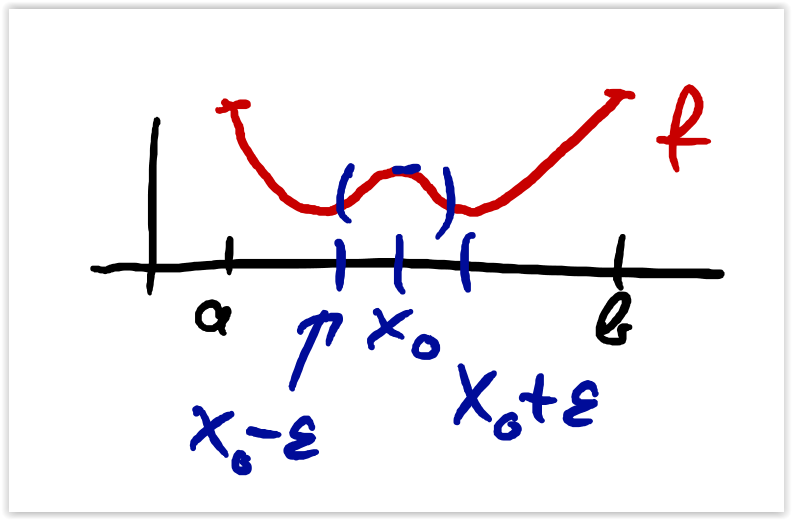
\includegraphics[width=0.3\textwidth]{mws_def.png}
	  \caption{Lokales Minimum/Maximum\protect\cite{HM12}}
	  \label{fig:mws_min_max}
	\end{figure}
  \begin{satz}
    Besitzt eine stetig diffbare Funktion $f: (a,b) \rightarrow \R$ in einer Stelle $x_0 \in (a,b)$ ein lokales Maximum oder Minimum, so gilt notwendigerweise $f'(x_0) = 0$.
  \end{satz}
  \begin{satz}
    Seien $f,g:[a,b] \rightarrow \R$ stetig und auf $(a,b)$ diffbar mit $g'(x) > 0$ bzw. $g'(x) <0$ jeweils für alöle $x \in (a,b)$. 
    \begin{itemize}
      \item[a) ] \textbf{Satz von Rolle:} Gilt $f(a) = f(b)$, so existiert ein $\xi \in (a,b)$ mit $f'(\xi) = 0$.
      \item[b) ] \textbf{1. Mittelwertsatz:} Es gibt ein $\xi \in (a,b)$ mit $f'(\xi) = \frac{f(b) - f(a)}{b-a}$.
      \item[c) ] \textbf{2. Mittelwertsatz:} Es gibt ein $\xi \in (a,b)$ mit $\frac{f'(\xi)}{g'(\xi)} = \frac{f(b) - f(a)}{g(b) - g(a)}$.
    \end{itemize}
  \end{satz}
  \begin{figure}[H] 
		\centering
		\begin{minipage}{.5\textwidth}
		  \centering
		  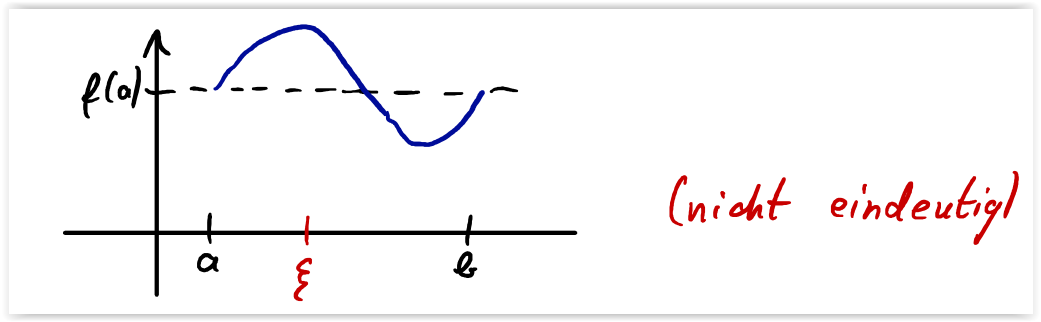
\includegraphics[width=0.8\linewidth]{mws_rolle.png}
		  \caption{Zu a) \protect\cite{HM12}}
		  \label{fig:mws_rolle}
		\end{minipage}%
		\begin{minipage}{.5\textwidth}
		  \centering
		  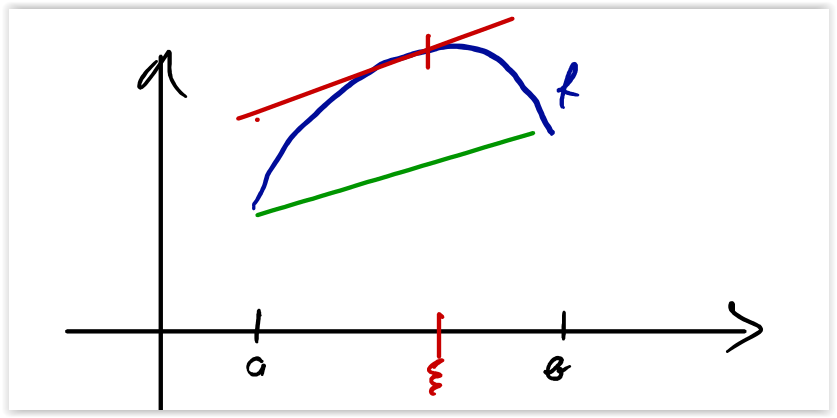
\includegraphics[width=0.8\linewidth]{mws_1.png}
		  \caption{Zu b) \protect\cite{HM12}}
		  \label{fig:funkt_sinh}
		\end{minipage}
  \end{figure}
		
  \subsection{Monotonie}	
  \begin{satz}$\;$ \newline
  \vspace{-0.5cm}
    \begin{itemize}
      \item[a) ] Ist $f:(a,b)\rightarrow \R$ differenzierbar und ist $f:[a,b]\rightarrow \R$ stetig und es gelte $f'(x_0) = 0 \quad \forall x \in (a,b)$, so ist $f$ konstant.
      \item[b) ] 
      \begin{tabular}{l c l} 
        $f'(x) \geq 0 \quad \forall x \in (a,b)$ & $\Leftrightarrow$ & $f$ ist monoton wachsend \\
        $f'(x) > 0 \quad \forall x \in (a,b)$ & $\Rightarrow$ & $f$ ist streng monoton wachsend \\
        $f'(x) \leq 0 \quad \forall x \in (a,b)$ & $\Leftrightarrow$ & $f$ ist monoton fallend \\
        $f'(x) < 0 \quad \forall x \in (a,b)$ & $\Rightarrow$ & $f$ ist streng monoton fallend \\
      \end{tabular}
    \end{itemize}
  \end{satz}	
  
  \subsection{Das Prinzip von l'Hospital}
  \begin{satz}
    Gilt $\lim\limits_{b\rightarrow a} f(b) = 0$, $\lim\limits_{b\rightarrow a} g(b) = 0$ und existiert $\lim\limits_{b\rightarrow a} \frac{f'(b)}{g'(b)}$, so existiert auch $\lim\limits_{b\rightarrow a} \frac{f(b)}{g(b)}$ und er ist gleich $\lim\limits_{b\rightarrow a} \frac{f'(b)}{g'(b)}$. Analog $\lim\limits_{b\rightarrow a} f(b) = \infty$ und $\lim\limits_{b\rightarrow a} g(b) = \infty$.
    \begin{equation}
      \Rightarrow \lim\limits_{b\rightarrow a} f(b) = 0 \land \lim\limits_{b\rightarrow a} g(b) = 0 \land \lim\limits_{b\rightarrow a} \frac{f'(b)}{g'(b)} \Rightarrow \lim\limits_{b\rightarrow a} \frac{f'(b)}{g'(b)} = \lim\limits_{b\rightarrow a} \frac{f(b)}{g(b)}
    \end{equation}
  \end{satz}
  \begin{bem}
    Zur Berechnung muss der Ausdruck gegebenenfalls auf $"\frac{0}{0}"$ zurückgeführt werden. Entspricht zum Beispiel $\frac{f(b)}{g(b)}$ der Form $"\frac{\infty}{\infty}"$ kann durch Umformung zu $\frac{\frac{1}{f(b)}}{\frac{1}{g(b)}}$ l'Hospital angewandt werden.\newline
    Liegt ein Ausdruck in der Form $"\infty \cdot 0"$ wie zum Beispiel $\lim\limits_{x\rightarrow \infty} \underbrace{x}_{\rightarrow \infty} \underbrace{ln\left(\frac{x+1}{x-1}\right)}_{\rightarrow 0 }$ vor, kann durch Umformung zu $\lim\limits_{x\rightarrow \infty} \frac{ln\left(\frac{x+1}{x-1}\right)}{\left(\frac{1}{x}\right)}$ wieder in die Form $"\frac{0}{0}"$ gebracht werden.
  \end{bem}
  \newpage
  
\section{Taylorpolynome}
  \begin{satz}
  Sei $f:I\rightarrow \R$ eine $C{n+1}$ Funktion und sei $x_0 \in I$ und heißt Entwicklungspunkt. Dann ist
  \begin{itemize}
    \item[a) ] das Taylorpolynom n-ten Grades zum Entwicklungspunkt $x_0$ gegebn durch
    \begin{equation}
    T_n(f, x, x^*) = \sum\limits_{k= 0}^n \frac{f^{(k)}(x^*)}{k!} (x-x^*)^k
    \end{equation}
    und stimmt mit $f$ in $x_0$ bis zur n-ten Ableitung überein.
    \item[b) ] Der Fehler 
    \begin{equation}
      R_n(x,x_0) = f(x) - T_n(x,x_0)
    \end{equation}
    ist gegeben durch die Restgliedformel nach Lagrange
    \begin{equation}
      R_n(x,x_0) = \frac{f^{(n+1)}(\xi)}{(n+1)!}(x-x_0)^{n+1}
    \end{equation}
    wobei $\xi = x_0 + \Theta (x-x_0)$ mit $\Theta \in (0,1)$, d.h. $\xi$ ist eine Zahl zwischen $x$ und $x_0$. Es gilt dann
    \begin{equation}
      \big|R_n(x,x_0)\big| = \frac{\sup\limits_{\xi \in (x_0,x)} \left|f^{(n+1)}(\xi)\right|}{(n+1)!}|x-x_0|^{(n+1)}
    \end{equation}
  \end{itemize}
  \end{satz}  
\newpage

\section{Reihen}
  \subsection{Satz von Bolzano-Weierstraß (Kompaktheitssatz)}
  \begin{satz}
    Jede beschränkte reelle Folge $(a_n)_{n \in \N}$ besitzt eine konvergente Teilfolge.
  \end{satz}
  \begin{bem}
    Im Prinzip unterteilt man das Intervall jeweils mittig und erhält so eine Folge von Teilintervalle mit je unendlich vielen Folgengliedern. Daraus konstruiert man eine konvergente Teilfolge
  \end{bem}  
  \begin{bem}
    Der Satz gilt auch im $\R^d$ aber nicht im $\R^{\infty}$.
  \end{bem}
  \begin{definition}
    $x$ heißt Häufungspunkt einer Folge $(a_n)_{n \in \N}$, wenn eine Teilfolge existiert, die gegen $x$ konvergiert.
  \end{definition}
  Formuliert man den Satz von Bolzano Weierstraß dahingehen um, lautet er
  \begin{bem}
    Jede beschränkte reelle Folge besitzt mindestens einen Häufungspunkt.
  \end{bem}
  \begin{definition}$\;$\newline 
    limes inferior$\;$: $\liminf\limits_{n\rightarrow \infty} a_n \;= \inf\lbrace x:\; x$ ist ein Häufungspunkt von $(a_n)_{n \in \N}\rbrace$ \newline
    limes superior: $\limsup\limits_{n\rightarrow \infty} a_n = \sup\lbrace x:\; x$ ist ein Häufungspunkt von $(a_n)_{n \in \N}\rbrace$
  \end{definition}
  
  \subsection{Häufungspunkte}
  \begin{bem}
    Ein Häufungspunkt $a$ einer Folge $(a_n)$ ist der Grenzwert einer Teilfolge $(a_{n_k})$.
    \begin{equation*}
      \lim\limits_{k \rightarrow \infty} a_{n_k} = a
    \end{equation*}
    \begin{tabular}{l c l}
      Größter HP&: & $\limsup_{n \rightarrow \infty} a_n = \overline{\lim\limits_{n \rightarrow \infty}} a_n$ \\
      Kleinster HP&: & $\liminf_{n \rightarrow \infty} a_n = \underline{\lim\limits_{n \rightarrow \infty}} a_n$
    \end{tabular} \newline
    Es gilt:
    \begin{align*}
    \textbf{(1)}\quad \overline{\lim\limits_{n \rightarrow \infty}} a_n &= \underline{\lim\limits_{n \rightarrow \infty}} a_n \Rightarrow a_n \text{ konvergiert} \\
    \textbf{(2)}\quad \lim\limits_{n \rightarrow \infty} a_n  &\rightarrow \text{ jede Teilfolge } a_{n_k} \text{ konvergiert.}
    \end{align*}
  \end{bem}  
  
  \subsection{Cauchy-Folgen}
  \begin{definition}
    Eine Folge $(a_n)_{n \in \N}$ heißt Cauchy-Folge, falls für alle $\varepsilon > 0$ ein $N \in \N$ \colRed{(im Script steht $n \in \N$, aber irgendwie unlogisch)} existiert, sodass für alle $m,n \in \N$ gilt: $|a_n - a_m|<\varepsilon$.
    \begin{equation}
      \forall \varepsilon > 0:\; \exists N\quad \forall n,m \geq N: |a_n -a_m| < \varepsilon 
    \end{equation}
    (vgl. Konvergenzkriterium \eqref{def:folge_konvergenz} bzw. \eqref{eq:folge_konvergenz}).
  \end{definition}
  \begin{satz}
    Jede konvergente Folge ist auch eine Cauchy-Folge.
  \end{satz}
  \begin{satz}
    In den reellen Zahlen gilt: Jede Cauchy-Folge inst konvergent.
  \end{satz}
  \begin{bem}
    Jede Cauchy-Folge ist beschränkt (somit ist Bolzano Weierstraß anwendbar).
  \end{bem}
  Die Konsequenzen aus dem Beweis der obigen Aussagen sind:
  \begin{bem} $\;$\newline \vspace{-0.5cm}
    \begin{itemize}
      \item Um Konvergenz nachzuweisen reicht der Nachweis einer Cauchy-Folge (Cauchy-Kriterium)
      \item Supremumsvollständigkeit $\Rightarrow$ Cauchyfolgenvollständigkeit
    \end{itemize}
  \end{bem}
  
  \subsection{Reihen reeller Zahlen}
  \begin{definition}
    Bildet man zu einer gegebenen Folge $(a_n)_{n \in \N}$ mit $a_n \in \R$ eine neue Folge $(s_n)_{n \in \N}$ mit 
    \begin{equation}
      s_n = \sum\limits_{k=0}^n a_k
    \end{equation}
    so wird die Folge $(s_n)_{n \in \N}$ eine Reihe genannt. Die einzelnen $s_n$ heißen Partialsummen der Reihe. Ist $(s_n)_{n \in \N}$ konvergent, so wird der Grenzwert $s = \lim\limits_{n\rightarrow \infty} \sum\limits_{k = 0}^n a_k$ mit $\sum\limits_{k=0}^{\infty} a_k$ bezeichnet. Oft wird $\sum\limits_{k=0}^{\infty} a_k$ als Abkürzung für $(s_n)_{n \in \N}$ verwendet.
  \end{definition}
  
  \begin{satz} $\;$\newline \vspace{-0.5cm}
  \begin{itemize}
  \item[a) ] Es gilt das Cauchysche Konvergenzkriterium.
    \begin{equation}
      \sum\limits_{k=0}^{\infty} a_k \; konvergent \; \Leftrightarrow \forall \varepsilon > 0 \quad \exists N \quad \forall n,m \geq N: \quad \left| \sum\limits_{k = n+1}^m a_k \right| < \varepsilon
    \end{equation}
    \item[b) ] Notwendige aber nicht hinreichende Bedingung für die Konvergenz von $\sum\limits_{k=0}^{\infty} a_k$ ist, dass $a_k$ eine Nullfolge ist, also das gilt: $\lim\limits_{k \rightarrow \infty} a_k = 0$
    \item[c) ] Sind 
    \begin{equation*}
      \sum\limits_{k=0}^{\infty} a_k, \qquad \sum\limits_{k=0}^{\infty} b_k
    \end{equation*}
    konvergente Reihen, so konvergieren auch
    \begin{align*}
    \sum\limits_{k=0}^{\infty} \left( a_k + b_k\right) &= \left(\sum\limits_{k=0}^{\infty} a_k\right) + \left(\sum\limits_{k=0}^{\infty} b_k\right) \\
    \sum\limits_{k=0}^{\infty} \left( \lambda a_k\right) &= \lambda \sum\limits_{k=0}^{\infty} a_k
    \end{align*}
  \end{itemize}
  \end{satz}
  
	  \subsubsection{Wichtige Reihen}
	  \begin{itemize}
	    \item Exponentialreihe:
	    \begin{equation}
	      e^x = \sum\limits_{k=0}^\infty \frac{x^k}{k!} \qquad \forall x \in \R
	    \end{equation}
	    \item Geometrische Reihe
	    \begin{equation}
	      \frac{1}{1-q} = \sum\limits_{k = 0}^\infty q^k \qquad |q| < 1
	    \end{equation}
	    \item Sinusreihe
	    \begin{equation}
	      sin(y) = \sum\limits_{k = 0}^\infty \frac{(-1)^k y^{2k+1}}{(2k+1)!} = y -\frac{1}{3!}y^3 + \frac{1}{5!}y^5 + ...
	    \end{equation}
	    \item Cosinusreihe
	    \begin{equation}
	      cos(y) = \sum\limits_{k = 0}^\infty = (-1)^k \frac{y^2k}{(2k)!} = 1 - \frac{1}{2}y^2 + \frac{1}{4!}y^4 + ...
	    \end{equation}
	  \end{itemize}
	  
	  \subsubsection{Konvergenzen und Divergenzen ausgewählter Reihen}
	  \begin{itemize}
	    \item Geometrische Reihe \newline
	    Konvergenz kann nur für $|q| < 1$ vorliegen da $a_k$ eine Nullfolge sein muss. Sonst divergent.
	    \item Harmonische Reihe \newline
	    \begin{equation}
	      \lim\limits_{n \rightarrow \infty} \sum\limits_{k = 0}^n \frac{1}{k} = \infty
	    \end{equation}
	  \end{itemize}
	  
	  \subsubsection{Leibnizkriterium für alternierende Reihen}
	  \begin{satz}
	    Ist $a_k \geq 0$ und ist $(a_k)_{k \in \N}$ monoton fallend, oder anders ausgedrückt ist $(a_k)_{k \in \N}$ eine monoton fallende Nullfolge, so ist
	    \begin{equation*}
	      \sum\limits_{k = 1}^{\infty} (-1)^k a_k
	    \end{equation*}
	    konvergent.
	  \end{satz}
  
  \subsection{Absolut konvergente Reihen}
  \begin{definition}
    Eine Reihe $\sum\limits_{k=0}^\infty$ heißt absolut konvergent, falls die Reihe $\sum\limits_{k=0}^\infty |a_k|$ konvergiert.
  \end{definition}
  \begin{satz}
    Jede absolut konvergente Reihe ist konvergent.
  \end{satz}
	  \subsubsection{Konvergenzkriterien}
	  \begin{satz}
	    \begin{itemize}
	      \item[a) ] Die absolute Konvergenz von $\sum\limits_{k=0}^\infty a_k$ ist äquivalent zur Beschränktheit von $\left(\sum\limits_{k=0}^\infty a_k \right)_{k\in \N}$.
	      \item[b) ] Majorantenkriterium \newline
	      Sei $|a_k| \leq b_k$ und $\sum\limits_{k=0}^\infty b_k$ konvergent, so folgt die absolute Konvergenz von $\sum\limits_{k=0}^\infty a_k$. Die Reihe $\sum\limits_{k=0}^\infty b_k$ heißt konvergente Majorante. 
	      \item[c) ] Divergenzkriterium \newline
	      Sei $0 \leq a_k \leq b_k$ und $\sum\limits_{k=0}^\infty a_k$ divergent (d.h. = $\infty$). Dann ist auch $\sum\limits_{k=0}^\infty b_k$ divergent und $\sum\limits_{k=0}^\infty a_k$ heißt divergente Minorante.
	    \end{itemize} \label{ax:reihe_konv_a}
	  \end{satz}
	  \begin{bem}
	    Zu \eqref{ax:reihe_konv_a} b): Häufig wird die geometrische Reihe als konvergente Majorante genutzt.
	  \end{bem}
	  \begin{satz}
	    Vergleichsreihe:
	    \begin{equation}
	      \sum\limits_{k = 1}^\infty \frac{1}{k^\alpha} 
	      \begin{cases}
	        \text{konvergiert für }\alpha > 1 \\
	        \text{divergiert für  }\;\;\alpha \leq 1
	      \end{cases}
	    \end{equation}
	  \end{satz}
	  \begin{satz}
	    Wurzelkriterium: Gegeben sei die Reihe $\sum\limits_{k=1}^\infty a_k$. Man setzt $\alpha = \limsup_{k \rightarrow \infty} |a_k|^{\frac{1}{k}}$.
	    \begin{itemize}
	      \item[a) ] Ist $\alpha < 1$, so konvergiert $\sum\limits_{k=1}^\infty a_k$ absolut.
	      \item[b) ] Ist $\alpha > 1$, so divergiert $\sum\limits_{k=1}^\infty a_k$.
	      \item[c) ] Ist $\alpha = 1$, so ist keine Aussage möglich.
	    \end{itemize}\label{ax:folgen_konv_wurzel}
	  \end{satz}
	  \begin{satz}
	    Quotientenkriterium: Gegeben sei $\sum\limits_{k=1}^\infty a_k$ mit $a_k \neq 0$ für $k \in \N$. Wir setzen $\underline{\alpha} = \liminf\limits_{k \rightarrow \infty} \left| \frac{a_{k+1}}{a_k}\right|$ und $\overline{\alpha} = \limsup\limits_{k \rightarrow \infty} \left| \frac{a_{k+1}}{a_k}\right|$.
	    \begin{itemize}
	      \item[a) ] Ist $\overline{\alpha} < 1$, so konvergiert $\sum\limits_{k=1}^\infty a_k$ absolut.
	      \item[b) ] Ist $\underline{\alpha} > 1$, so divergiert $\sum\limits_{k=1}^\infty a_k$.
	    \end{itemize}\label{ax:folgen_konv_quot}
	  \end{satz}
    \begin{bem}
      Das Wurzelkriterium \eqref{ax:folgen_konv_wurzel} wird häufig bei n-ten Wurzeln angewandt, das Quotientenkriterium \eqref{ax:folgen_konv_quot} häufig bei Fakultäten.
    \end{bem}
  \subsection{Umordnung von Reihen}
  \begin{satz}
    Umordnung absolut konvergenter Reihen: Sei $\sigma: \N_0 \rightarrow \N_0$ eine bijektive Abbildung (erzeugt Umnummerierung der Folgenglieder). Ist $\sum\limits_{k=0}^\infty a_k$ absolut konvergent, so ist auch jede umgeordnete Reihe $\sum\limits_{k=0}^\infty a_{\sigma_k}$ absolut konvergent und es gilt
    \begin{equation}
      \sum\limits_{k=0}^\infty a_k = \sum\limits_{k=0}^\infty a_{\sigma_k}
    \end{equation}
  \end{satz}
  \begin{satz}
    Seien $\sum\limits_{k=0}^\infty a_k$ und $\sum\limits_{k=0}^\infty b_m$ absolut konvergent. Dann ist die Reihe $\sum\limits_{k=0}^\infty a_{\sigma_k} b_{\mu_k}$ für jede Nummerierung: $(\sigma,\mu):(\N_0 \rightarrow \N_0^2$ mit $k \rightarrow (\sigma_k, \mu_k)$ absolut konvergent und es gilt
    \begin{equation}
      \sum\limits_{k=0}^\infty a_{\sigma_k} b_{\mu_k} = \left(\sum\limits_{k=0}^\infty a_k \right) =  \left(\sum\limits_{k=0}^\infty b_m \right)
    \end{equation}
  \end{satz}
  
  \subsection{Potenzreihen}
  \begin{definition}
    Eine Reihe der Form $\sum\limits_{k = 0}^\infty a_k(z-z_0)^k$ heißt Potenzreihe.
  \end{definition}
	  \subsubsection{Taylorreihe}
	  Ist eine Funktion unendlich oft diffbar kann aus dem Taylorpolynom $T_n(x,x_0)$ für $n\rightarrow \infty$ die sogenannte Taylorreihe
	  \begin{equation}
	   T_\infty (x,x_0) = \sum\limits_{k = 0}^\infty \frac{f^{(k)}(x_0)}{k!}(x-x_0)^k
	  \end{equation}
	  erhalten werden.
	  \begin{satz}
	    Die Taylorreihe $T_\infty(f,x,x_0)$ konvergiert in $x \in \R$ genau dann gegen $f(x)$, falls
	    \begin{equation*}
	      \lim\limits_{n \rightarrow \infty} R_n(f,x,x_0) = 0
	    \end{equation*}
	  \end{satz}
	  \begin{satz}
	    Identitätssatz:
	    \begin{align}
	      \text{Taylorreihe: } f(x) &= \sum\limits_{k = 0}^\infty \frac{f^{(k)}(x_0)}{k!}(x-x_0)^k \nonumber \\
	      \text{Potenzreihe: } f(x) &= \sum\limits_{k = 0}^\infty a_k (x-x_0)^k \nonumber \\
	      &\Rightarrow a_k = \frac{f^{(k)}x_0}{k!}
	    \end{align}
	  \end{satz}
	  \subsubsection{Konvergenz der Potenzreihen}
	  \begin{satz}$\;$ \newline \vspace{-0.5cm}
	    \begin{itemize}
	      \item[a) ] Zu jeder Potenzreihe $\sum\limits_{k = 0}^\infty a_k(z-z_0)^k$ gibt es eine Zahl $r \in [0,\infty]$, den sogenannten Konvergenzradius der Potenzreihe, mit der Eigenschaft, dass $\sum\limits_{k = 0}^\infty a_k(z-z_0)^k$ absolut konvergent für $|z-z_0| < r$ ist und divergent für $|z-z_0| > r$.
	      \item[b) ] Für den Konvergenzradius gilt die Formel von Cauchy-Hadamard:
	      \begin{equation}
	        r = \frac{1}{\limsup\limits_{k \rightarrow \infty} |a_k|^\frac{1}{k}}
	      \end{equation}
	      wobei $\frac{1}{\infty}=0$ und $\frac{1}{0} = \infty$ gesetzt wird.
	    \end{itemize}
	    Dazu:
	    \begin{figure}[H] 
				\centering
				\begin{minipage}{.5\textwidth}
				  \centering
				  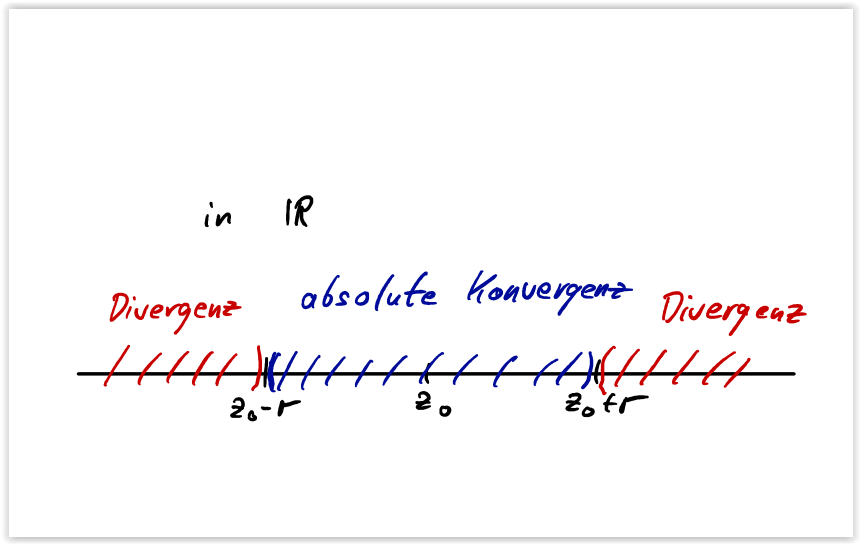
\includegraphics[width=0.8\linewidth]{reihen_potenzreihen_r.png}
				  \caption{Potenzradius in $\R$ \protect\cite{HM12}}
				  \label{fig:reihe_potenzradius_r}
				\end{minipage}%
				\begin{minipage}{.5\textwidth}
				  \centering
				  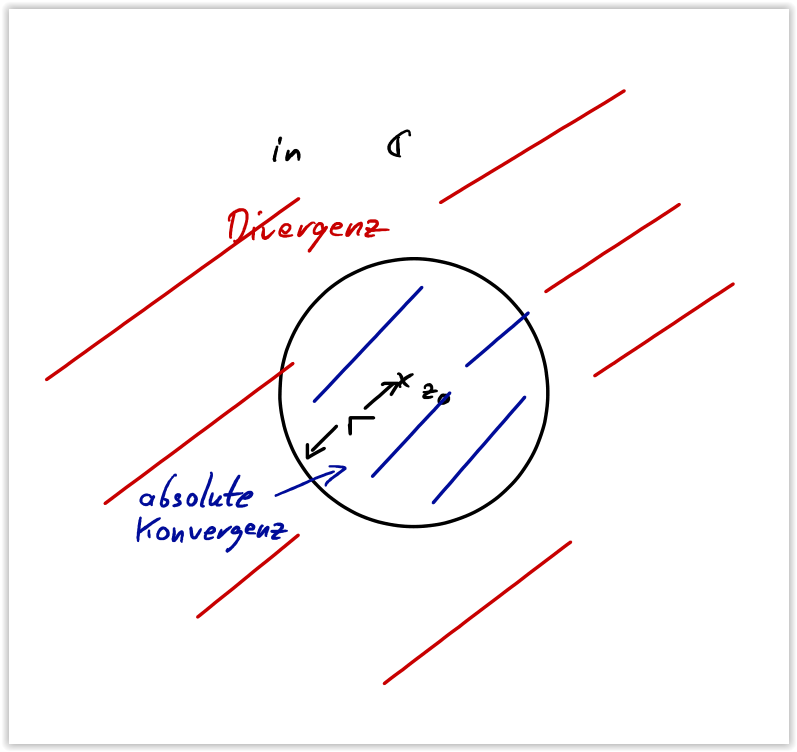
\includegraphics[width=0.55\linewidth]{reihen_potenzreihen_c.png}
				  \caption{Potenzradius in $\C$ \protect\cite{HM12}}
				  \label{fig:reihe_potenzradius_c}
				\end{minipage}
      \end{figure}
	  \end{satz}
    \begin{bem}
      Falls einer der folgenden Grenzwerte existiert bzw. $\infty$ ist, ist er gleich dem Konvergenzradius.
      \begin{equation*}
        r = \frac{1}{\lim |a_k|^\frac{1}{k}} \quad bzw. \quad r = \lim\limits_{k \rightarrow \infty} \left| \frac{a_k}{a_{k+1}}\right|
      \end{equation*}
    \end{bem}	  
    \begin{bem}
      Da absolute Konvergenz vorliegt, können Potenzreiuhen miteinander multipliziert werden. Der Konvergenzradius ist mindestens so groß wie das Minimum der Konvergenzradien.
    \end{bem}
	  \begin{bem}
	    Potenzreihen sind innerhalb ihres Konvergenzradius beliebig oft diffbar und können gliedweise abgeleitet werden.
	  \end{bem}
	  \begin{satz}
	    Die formal abgeleitete Reihe $\sum\limits_{k = 1}^\infty a_k kx^{k-1}$ hat den gleichen Konvergenzradius wie die Ausgangsreihe.
	  \end{satz}
	  \begin{satz}
	    Es sei $\sum\limits_{k=0}\infty a_k x^k$ eine Potenzreihe mit Konvergenzradius $1$. Ist die Reihe auch in $x = 1$ konvergent, d.h. konvergiert $\sum\limits_{k = 0}^\infty$, so gilt
	    \begin{equation}
	      \lim\limits_{x\rightarrow 1} \sum\limits_{k = 0}^\infty a_k x^k = \sum\limits_ {k = 0}^\infty a_k
	    \end{equation}
	  \end{satz}
\newpage	  
	  
\section{Stetigkeit}
  \begin{definition}
    \textbf{A:} \newline Eine Funktion $f:D\rightarrow \R$ mit $D \subset \R$ heißt stetig in $x^* \in D$, falls $\lim\limits_{x \rightarrow x^*} f(x) = f(x^*)$. \label{def:stet_a}
  \end{definition}
  \begin{bem}
    Jede in $x^*$ differenzierbare Funktion ist auch stetig in $x^*$.
  \end{bem}
  \begin{definition}
    Eine Funktion $f:D\rightarrow \R$ mit $D \subset \R$ heißt stetig, falls $f$ stetig für alle $x^* \in D$ ist.
  \end{definition}
  \begin{satz}
    Sind $f$, $g$ stetige Funktionen und $\lambda \in \R$, so sind innerhalb ihres Definitionsbereich auch $\lambda f$, $f+g$, $f\cdot g$, $f\circ g$, $\frac{f}{g}$ stetige Funktionen.
  \end{satz}
  \begin{satz}
  Stetige Fortsetzbarkeit: Eine Definitionslücke einer gebrochen rationalen Funktion ist hebbar, wenn die Vielfachheit der Nullstelle $x_0$ im Zäherpolynom $\geq$ der Vielfachheit der Nullstelle $x_0$ im Nennerpolynom ist.
  \end{satz}
  \subsection{Arten von Unstetigkeiten}
  \begin{figure}[H] 
		\centering
		\begin{minipage}{.5\textwidth}
		  \centering
		  \captionsetup{justification=centering}
		  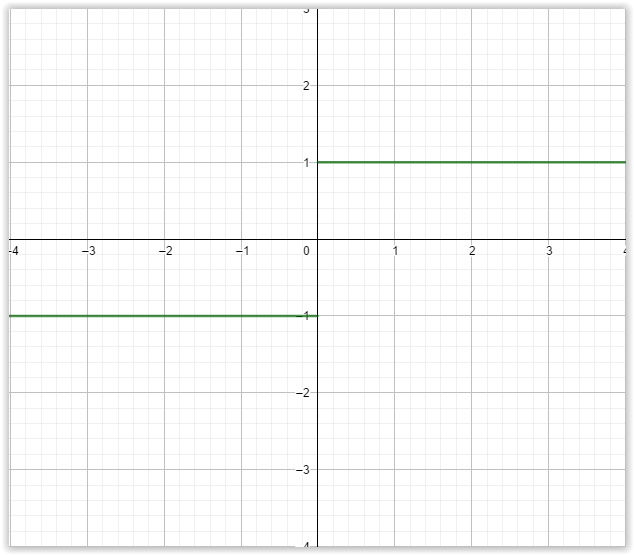
\includegraphics[width=0.78\linewidth]{stetigkeit_sprung.png}
		  \caption{$f(x) = \frac{|x|}{x}$ \\ (Sprungstelle)}
		  \label{fig:stetigkeit_sprung}
		\end{minipage}%
		\begin{minipage}{.5\textwidth}
		  \centering
		  \captionsetup{justification=centering}
		  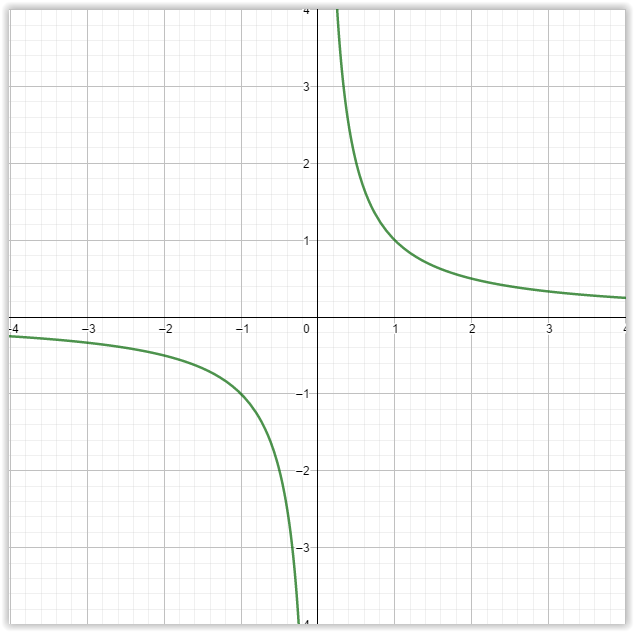
\includegraphics[width=0.7\linewidth]{stetigkeit_pol.png}
		  \caption{$f(x) = \frac{1}{x}$ \\ (Polstelle)}
		  \label{fig:stetigkeit_pol}
		\end{minipage}
  \end{figure}
  \begin{figure}[H] 
		\centering
	  \centering
	  \captionsetup{justification=centering}
	  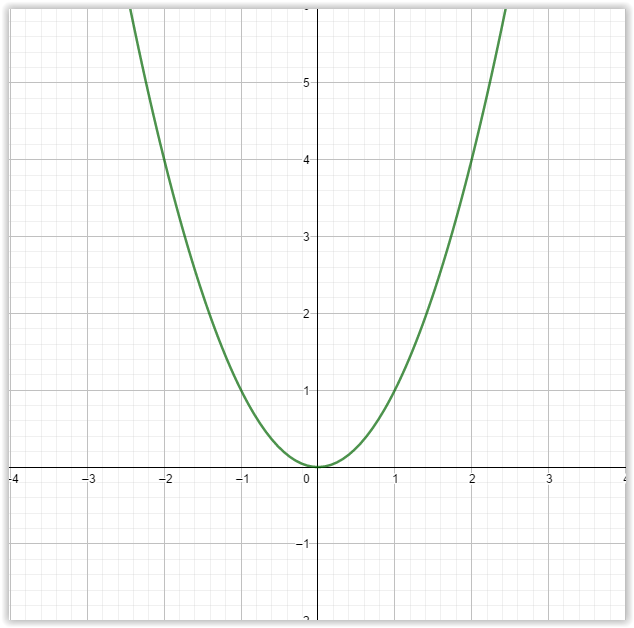
\includegraphics[width=0.35\linewidth]{stetigkeit_luecke.png}
	  \caption{$f(x) = \frac{x^3}{x}$ \\ (Lücke)}
	  \label{fig:stetigkeit_luecke}
  \end{figure}
  \begin{definition}
    $f:D\rightarrow \R$, $f(x)$ ist stetig in $x_0 \in D$ falls \newline
    \begin{itemize}
      \item[1) ] Falls z.z. ist dass $f$ stetig ist:
      \begin{equation}
        \forall \varepsilon > 0 \quad \exists \delta_\varepsilon \quad \forall x \in D: \left(|x-x_0| < \delta_\varepsilon \Rightarrow |f(x) - f(x_0)| < \varepsilon \right)
      \end{equation}
      \item[2) ] Falls z.z. ist dass $f$ nicht stetig ist:
      \begin{equation}
        \forall \text{ Folgen } (x_n) \text{ mit }x_n \rightarrow x_0 \text{ für }n \rightarrow \infty \Rightarrow f(x_n) \rightarrow f(x_0) \text{ für } n \rightarrow \infty.
      \end{equation}
      \item[2) ] 
      \begin{equation}
        \lim\limits_{x \rightarrow x_o^-} f(x) = \lim\limits_{x \rightarrow x_o^+} f(x)
        \end{equation}
    \end{itemize}
  \end{definition}
  \subsection{Nullstellensatz und Zwischenwertsatz}
  \begin{satz}
    Es sei $f: [a,b]\rightarrow \R§$ eine stetige Funktion. Dann gilt:
    \begin{itemize}
      \item[a) ] Es sei $f(a)f(b) < 0$. Dann existiert ein $x^*\in(a,b)$ mit $f(x^*) = 0$, d.h. eine Nullstelle von $f$.
      \item[b) ] Sei $f(a) < c < f(b)$. Dann existiert ein $x^* \in (a,b)$ mit $f(x^*) = c$.
    \end{itemize}
    \begin{figure}[H] 
			\centering
			\begin{minipage}{.5\textwidth}
			  \centering
			  \captionsetup{justification=centering}
			  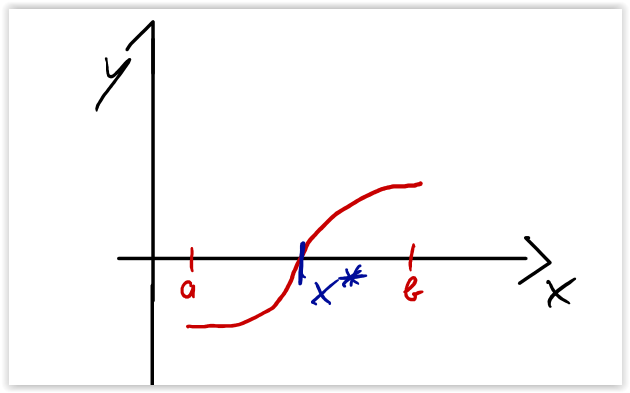
\includegraphics[width=0.75\linewidth]{potenzreihen_nullstellensatz.png}
			  \caption{Zu a) \\ (Nullstellensatz) \protect\cite{HM12}}
			  \label{fig:reihe_potenzradius_r}
			\end{minipage}%
			\begin{minipage}{.5\textwidth}
			  \centering
			  \captionsetup{justification=centering}
			  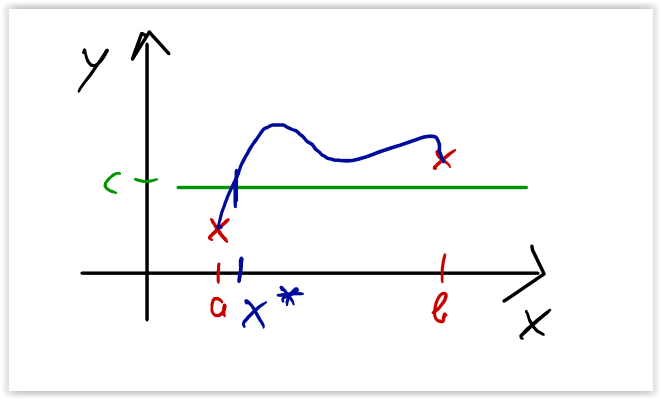
\includegraphics[width=0.8\linewidth]{potenzreihen_zwischenwertsatz.png}
			  \caption{Zu b) \\ (Zwischenwertsatz) \protect\cite{HM12}}
			  \label{fig:reihe_potenzradius_c}
			\end{minipage}
    \end{figure}
  \end{satz}
  \subsubsection{Sätze zu Stetigkeit und Monotonie}
  \begin{satz}
    $f:[a,b] \rightarrow \R$ sei streng monoton wachsend und  stetig. Dann existiert die Umkehrfunktion $f^{-1}:[f(a),f(b)]\rightarrow \R$. Diese ist streng monoton wachsend und stetig.
  \end{satz}
  \begin{definition}
    \textbf{B: ($\varepsilon -\delta$ Definition)} \newline
    Se $f:D\rightarrow \R$ mit $D \subset \R$. Dann heißt $f$ stetig in $x^*$, wenn für alle $\varepsilon > 0$ ein $\delta > 0$ existiert, sodass gilt: 
    \begin{equation}
      \forall x \in D:\quad |x - x^*| < \delta \Rightarrow |f(x) - f(x^*)| < \varepsilon
    \end{equation}
    Es muss zu jeder beliebig kleinen Seitenlänge $\varepsilon$ immer ein Rechteck mit Mitte $x^*$ existieren, sodass $f$ das Rechteck an den Seiten verlässt.
    \begin{figure}[H] 
			\centering
			\captionsetup{justification=centering}
			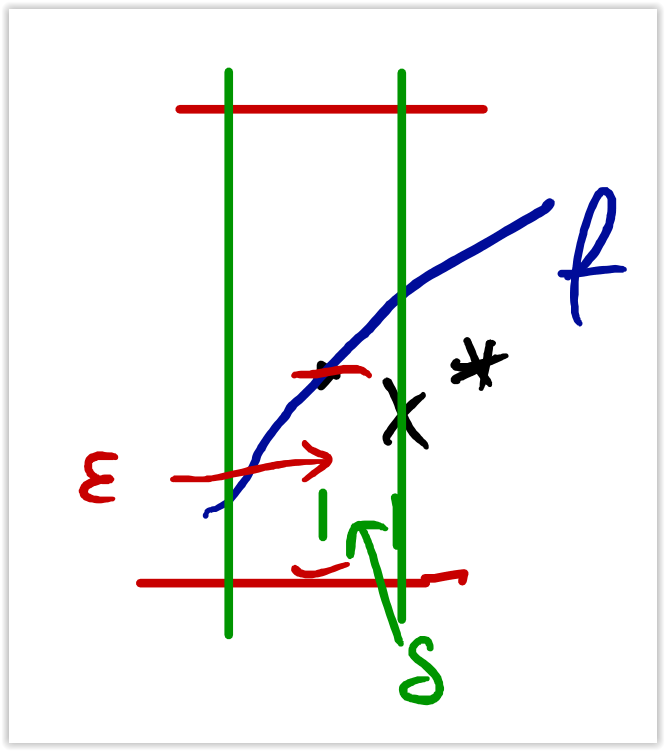
\includegraphics[width=0.2\linewidth]{stetigkeit_eps_del.png}
			\caption{$\varepsilon - \delta$ Kriterium \protect\cite{HM12}}
			\label{fig:stetigkeit_eps_del}
    \end{figure} \label{def:stet_b}
  \end{definition}
  
  \begin{definition}
    \begin{itemize}
      \item[a) ] $f$ heißt Lipschitz-stetig in $x^*$, wenn es ein $L > 0$ und $\delta > 0$ gibt, sodass für $x \in D$ mit $|x-x^*| < \delta$
	      \begin{equation}
	        |f(x) - f(x^*) \leq L|x-x^*|
	      \end{equation}
	      gilt.
      \item[b) ] $f$ heißt Hölder-stetig mit Exponent $\alpha \in (0,1]$, falls
	      \begin{equation}
	        |f(x) - f(x^*)| \leq L(|x-x^*|^\alpha
	      \end{equation}
	      gilt.
    \end{itemize}
    \begin{figure}[H] 
			\centering
			\begin{minipage}{.5\textwidth}
			  \centering
			  \captionsetup{justification=centering}
			  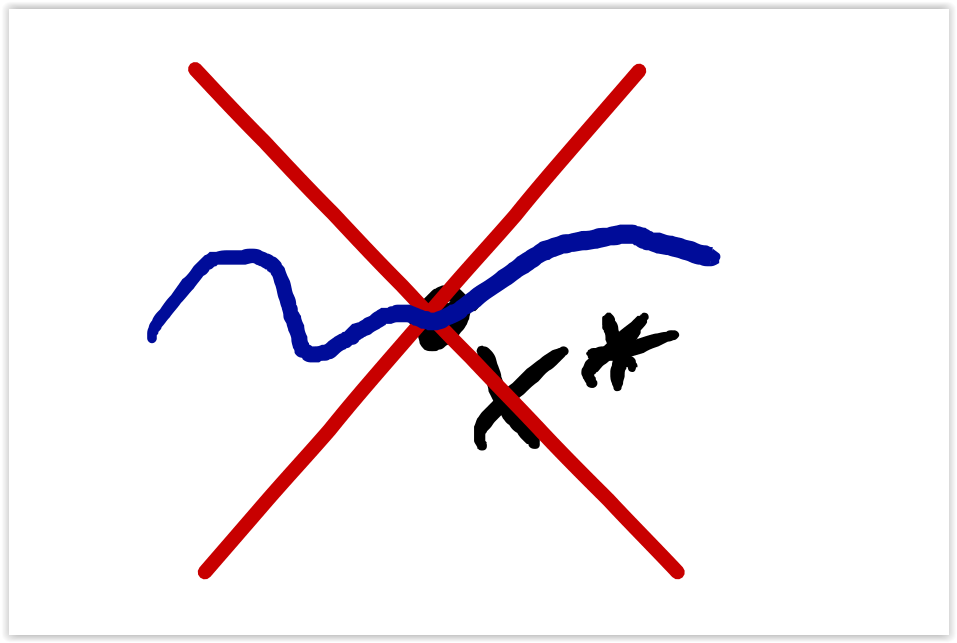
\includegraphics[width=0.9\linewidth]{stetigkeit_lipschitz.png}
			  \caption{Zu a) \\ (Lipschitzstetigkeit) \protect\cite{HM12}}
			  \label{fig:stetigkeit_lipschitz}
			\end{minipage}%
			\begin{minipage}{.5\textwidth}
			  \centering
			  \captionsetup{justification=centering}
			  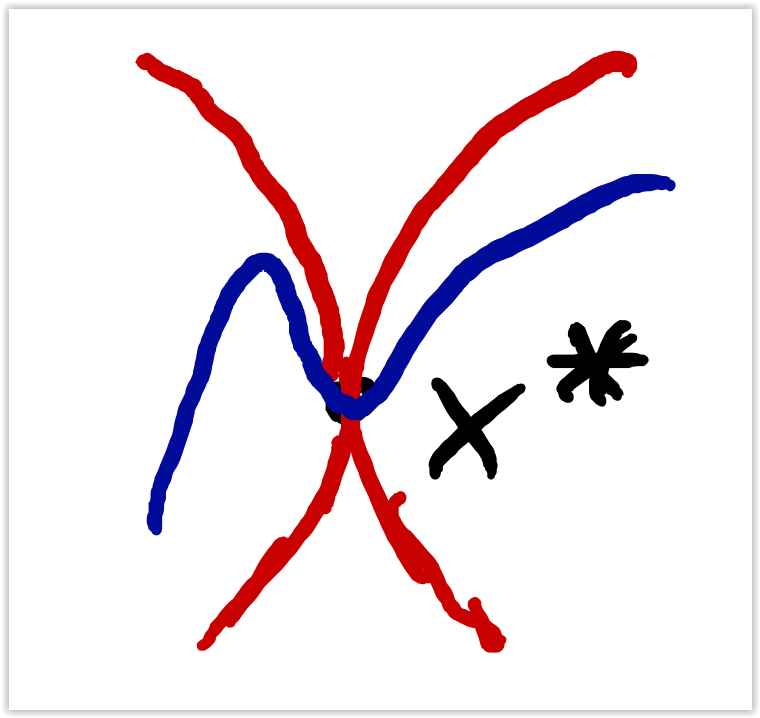
\includegraphics[width=0.65\linewidth]{stetigkeit_hoelder.png}
			  \caption{Zu b) \\ (Hölder-Stetigkeit) \protect\cite{HM12}}
			  \label{fig:stetigkeit_hoelder}
			\end{minipage}
    \end{figure}
  \end{definition}
  \begin{bem}
  \textbf{Zu a)}
    Es ist die Idee, eine Sekante so in den Graph zu legen, dass sie zwei Punkte des Graphen schneidet. Existiert nun eine Sprungstelle, so kann man diese Bedingung einhalten und die Steigung der Sektanten gegen unendlich treiben (praktisch eine senkrechte gerade). Liegt keine Sprungstelle vor, so wird die Steigung unter Einhaltung der Bedingung immer kleiner unendlich sein. Die Schranke für die Steigung ist hier $L$.
  \end{bem}
  \begin{satz}
    Definition A \eqref{def:stet_a} und Definition B \eqref{def:stet_b} der Stetigkeit sind äquivalent.
  \end{satz}
  \begin{definition}
    Eine Funktion $f:D\rightarrow \R$ mit $D \subset \R$ heißt Hölder- bzw. Lipschitzstetig, falls $f$ Hölder- bzw. Lipschitzstetig in jedem $x^* \in D$ ist. \newline
    Bezeichnungen: $C^{0,\alpha}$ steht für Hölder-stetig, $C^{0,1} = Lip$ steht für Lipschitzstetig.
  \end{definition}
  \begin{bem}
    Es gilt:
    \begin{equation}
      \text{differenzierbar } \Rightarrow \text{Lipschitzstetig } \Rightarrow \text{Hölder-stetig } \Rightarrow \text{stetig }
    \end{equation}
  \end{bem}    
  \newpage 
  
\section{Extremalprobleme}
Es sei $f:\R \rightarrow \R$, dann ist $f'(x^*) = 0$ notenwide Bedingung dafür, dass ein Minimum oder Maximum vorliegt, sofern $f$ diffbar ist.
\begin{satz}
  \textbf{Globale Theorie: } $[a,b]$ sei ein abgeschlossenes Intervall. $f:[a,b] \rightarrow \R$ sei stetig. Dann gibt es je ein $\underline{x}, \overline{x} \in [a,b]$ mit $f(\underline{x}) = \min\limits_{x \in [a,b]}f(x)$ und $f(\overline{x}) = \max\limits_{x \in [a,b]}f(x)$.\label{ax:extrema_global}
\end{satz}
\begin{bem} (Zu \eqref{ax:extrema_global})
  Stetige Funktionen auf kompakten Mengen nehmen das Maximum und Minimum an.
\end{bem}
\begin{satz}
  \textbf{Lokale Theorie: } Sei $f:[a,b] \rightarrow \R$ mit $f\in \C^3$ (also 3 mal stetig diffbar). Für $x* \in (a,b)$ gilt dann:
  \begin{itemize}
    \item[a) ] Aus $f'(x^*) = 0$ und $f''(x^*) > 0$ folgt, dass $f$ in $x^*$ ein lokales Minimum hat.
    \item[b) ] Aus $f'(x^*) = 0$ und $f''(x^*) < 0$ folgt, dass $f$ in $x^*$ ein lokales Maximum hat.
  \end{itemize}
\end{satz}
\newpage

\section{Funktionenfolgen}
\begin{definition}
  Eine Funtionenfolge ist allgemein eine Folge von Funktionen $f_1, f_2, ...$ bei denen alle Funktion dieselbe Definitions- und Zielmenge haben.
  \begin{equation}
  f:D\times \N \rightarrow Z, \quad (x,n) \rightarrow f_n(x)
  \end{equation}
  Wobei $D$ die Definitionsmenge und $Z$ die Zielmenge ist.
\end{definition}
\begin{definition}
  \begin{itemize}
    \item[a )] Eine Folge von Funktionen $f_n$ mit $f_n: D \rightarrow \R$ mit $D \subset \R$ heißt für $n \rightarrow \infty$ punktweise gegen $f$ konvergent, falls für alle $x \in D: \lim\limits_{n \rightarrow \infty} f_n(x) = f(x)$ gilt.
    \item[b )] Eine Funktionenfolge heißt gleichmäßig konvergent, falls \newline $\lim\limits_{n \rightarrow \infty} \sup\limits_{x \in D} |f_n(x) -f(x)| = 0$ gilt.
  \end{itemize}
  \begin{figure}[H] 
		\centering
	  \centering
	  \captionsetup{justification=centering}
	  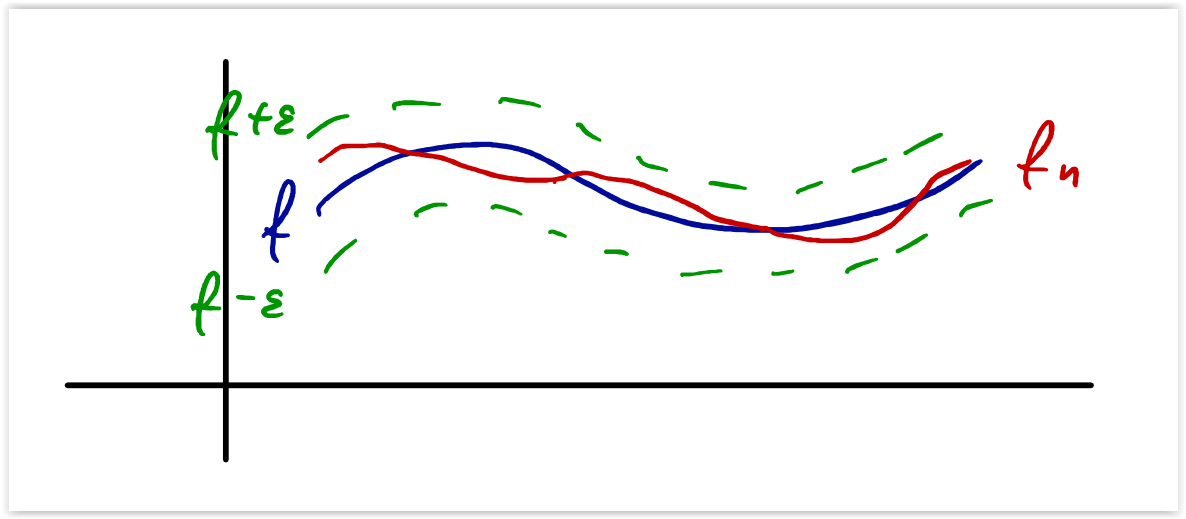
\includegraphics[width=0.5\linewidth]{funktionenfolgen_konvergenz.png}
	  \caption{Epsilonkanal Funktionenfolge \protect\cite{HM12}}
	  \label{fig:funktionenfolge_konvergenz}
  \end{figure}
\end{definition}
\begin{satz}
  Gegeben sei eine Folge stetiger Funktionen mit $f_n: D\rightarrow \R$. Gilt $f_n \rightarrow f$ gleichmäßig auf $D$, so ist auch die Grenzfunktion stetig.
\end{satz}
\begin{satz}
  Zu jeder Potenzreihe gibt es den Konvergenzradius $r$ mit $0 \leq r \leq \infty$ mit der Eigenschaft, dass $\sum\limits_{k=0}^\infty a_k(z-z_0)^k$ absolut konvergent für $|z-z_0| < r$ und divergent für $|z-z_0|>r$ ist.\newline
  Ferner konvergiert die Potenzreihe auf jeder Kreisscheibe $|z-z_0| < \delta$ mit $\delta < r$ auch gleichmäßig. 
\end{satz}
\begin{bem}
  Die Konsequenz aus obigem Satz ist, dass Potenzreihen für alle $z$ mit $|z-z_0| < r$ stetig sind.
\end{bem}
\begin{satz}
  $(f_n)_{n \in \N}$ seien auf $[a,b]$ differenzierbar. Für ein $x_0 \in [a,b]$ sei $f_n(x_0)$ konvergent. Ferner konvergiere $(f'_n)_{n \in \N}$ gleichmäßig (gegen $g$) auf $[a,b]$. Dann gilt:
  \begin{itemize}
    \item[1) ] $(f_n)_{n \in \N}$ konvergiert auf $[a,b]$ gleichmäßig.
    \item[2) ] $f(x) = \lim\limits_{n \rightarrow \infty} f_n(x)$ ist differenzierbar auf $[a,b]$ und es gilt $f'(x) = \lim\limits_{n \rightarrow \infty} f_n'(x)$ (und es gilt $f' = g$).
  \end{itemize}
\end{satz}
\begin{bem}
  Die Konsequenz aus obigem Satz ist, dass Potenzreihen innerhalb ihres Konvergenzradius beliebig oft differenzierbar sind und gliedweise abgeleitet werden können.
\end{bem}

\newpage  

\section{Nachwort}
Dieses Dokument versteht sich einzig als Zusammenfassung der Vorlesungsunterlagen aus der HM1-2 Vorlesung von Prof. Dr. Guido Schneider mit einigen zusätzlichen Beispielen. Der Sinn ist einzig mir selbst und meinen Kommilitonen das studieren der Mathematik zu erleichtern. In diesem Sinne erhebe ich keinerlei Anspruch auf das hier dargestellte Wissen, da es sich in großen Teilen nur um Neuformulierungen aus der Vorlesung und aus dem Begleitkurs vom Mint Kolleg handelt, in dem Frau Dr. Monika Schulz den Stoff bereits hervorragend zusammengefasst hat. Sollten sich einige Fehler eingeschlichen haben (was sehr wahrscheinlich ist) würde ich mich freuen, wenn man mir das kurz mitteilen würde damit ich eine Korrektur vornehmen kann. Das kann entweder über die Fachschaft erfolgen, oder gerne per E-Mail an f.leuze@outlook.de.

\bibliography{lit}

\end{document}